\section{Results}


\subsection{Part 1}
%%%%%%%%%%%%%%%%%%%%%%%%%%%%%%%%%%%%%%%%%%%%%%%%%%%%%%%%%%%%%%%%%%%%%%%%%%%%%%%%%%%%%%%%%%%%

%%%%                                PART 1 PROBLEM 3

%%%%%%%%%%%%%%%%%%%%%%%%%%%%%%%%%%%%%%%%%%%%%%%%%%%%%%%%%%%%%%%%%%%%%%%%%%%%%%%%%%%%%%%%%%%%
\subsubsection{Problem 3}
When steering the helicopter using only feed forward control from the joystick, it is extremely difficult to control. The mathematical models seem to represent the physical system quite well although forces from friction, air resistance, unlinearity in the motors etc. are not included. Also our propellers seemed to have a slight difference in weight causing the pitch to increase without any differential input.

We observed that the linearized model, as expected, did not represent the system very well outside of the linearized area. For example he helicopter needed a higher voltage in order to maintain its elevation the higher it was. 

%%%%%%%%%%%%%%%%%%%%%%%%%%%%%%%%%%%%%%%%%%%%%%%%%%%%%%%%%%%%%%%%%%%%%%%%%%%%%%%%%%%%%%%%%%%%

%%%%                                PART 1 PROBLEM 4

%%%%%%%%%%%%%%%%%%%%%%%%%%%%%%%%%%%%%%%%%%%%%%%%%%%%%%%%%%%%%%%%%%%%%%%%%%%%%%%%%%%%%%%%%%%%
\subsubsection{Problem 4}
Considering that our linearized model works best around the quilibrium, $0$ elevation, we need to alter the encoders in our system to count the equilibrium as $0$. We did this by adding constants to the encoder outputs, so that the equilibrium matched $0$ on the output.

We also had to find $V_s^\ast$, which is the $V_s$ input required to keep the helicopter at an elevation that matched the new encoder $0$. $V_s^\ast$ is added to the output from the controller, and was found by measuring the required voltage.

\begin{table}[h!]
	\centering
	\caption{Measured values.}
	\begin{tabular}{lrl}
		\toprule
		Variable & Value & Unit\\
		\midrule
	    Elevation encoder offset   & $-32$ & \degree  \\
		Pitch encoder offset & $-4.1$      & \degree  \\
		$V_s^\ast$   &  $\; 6.7$           & \volt    \\
		\bottomrule
	\end{tabular}
\label{tab:offsets}
\end{table}

Combining the equations for motor voltage and momentum around the elevation joint, and inserting $V_s^\ast$ gives the motor force constant, $K_f$

\begin{equation}
    K_f = \frac{(m_c l_c - 2 m_p l_h)g}{V_s l_h}
\end{equation}

Inserted values give $K_f = 0.149N/V$.

\subsection{Part 2}
%%%%%%%%%%%%%%%%%%%%%%%%%%%%%%%%%%%%%%%%%%%%%%%%%%%%%%%%%%%%%%%%%%%%%%%%%%%%%%%%%%%%%%%%%%%%

%%%%                                PART 2 PROBLEM 1

%%%%%%%%%%%%%%%%%%%%%%%%%%%%%%%%%%%%%%%%%%%%%%%%%%%%%%%%%%%%%%%%%%%%%%%%%%%%%%%%%%%%%%%%%%%%
\subsubsection{Problem 1}
We added a PD controller for the pitch to Simulink, as shown in Figure \ref{fig:simulink_pitch} and \ref{fig:simulink_pitch_controller}.
%Simulink:
\begin{figure}[htb]
	\centering
	\begin{minipage}{.45\textwidth}
	    \centering
		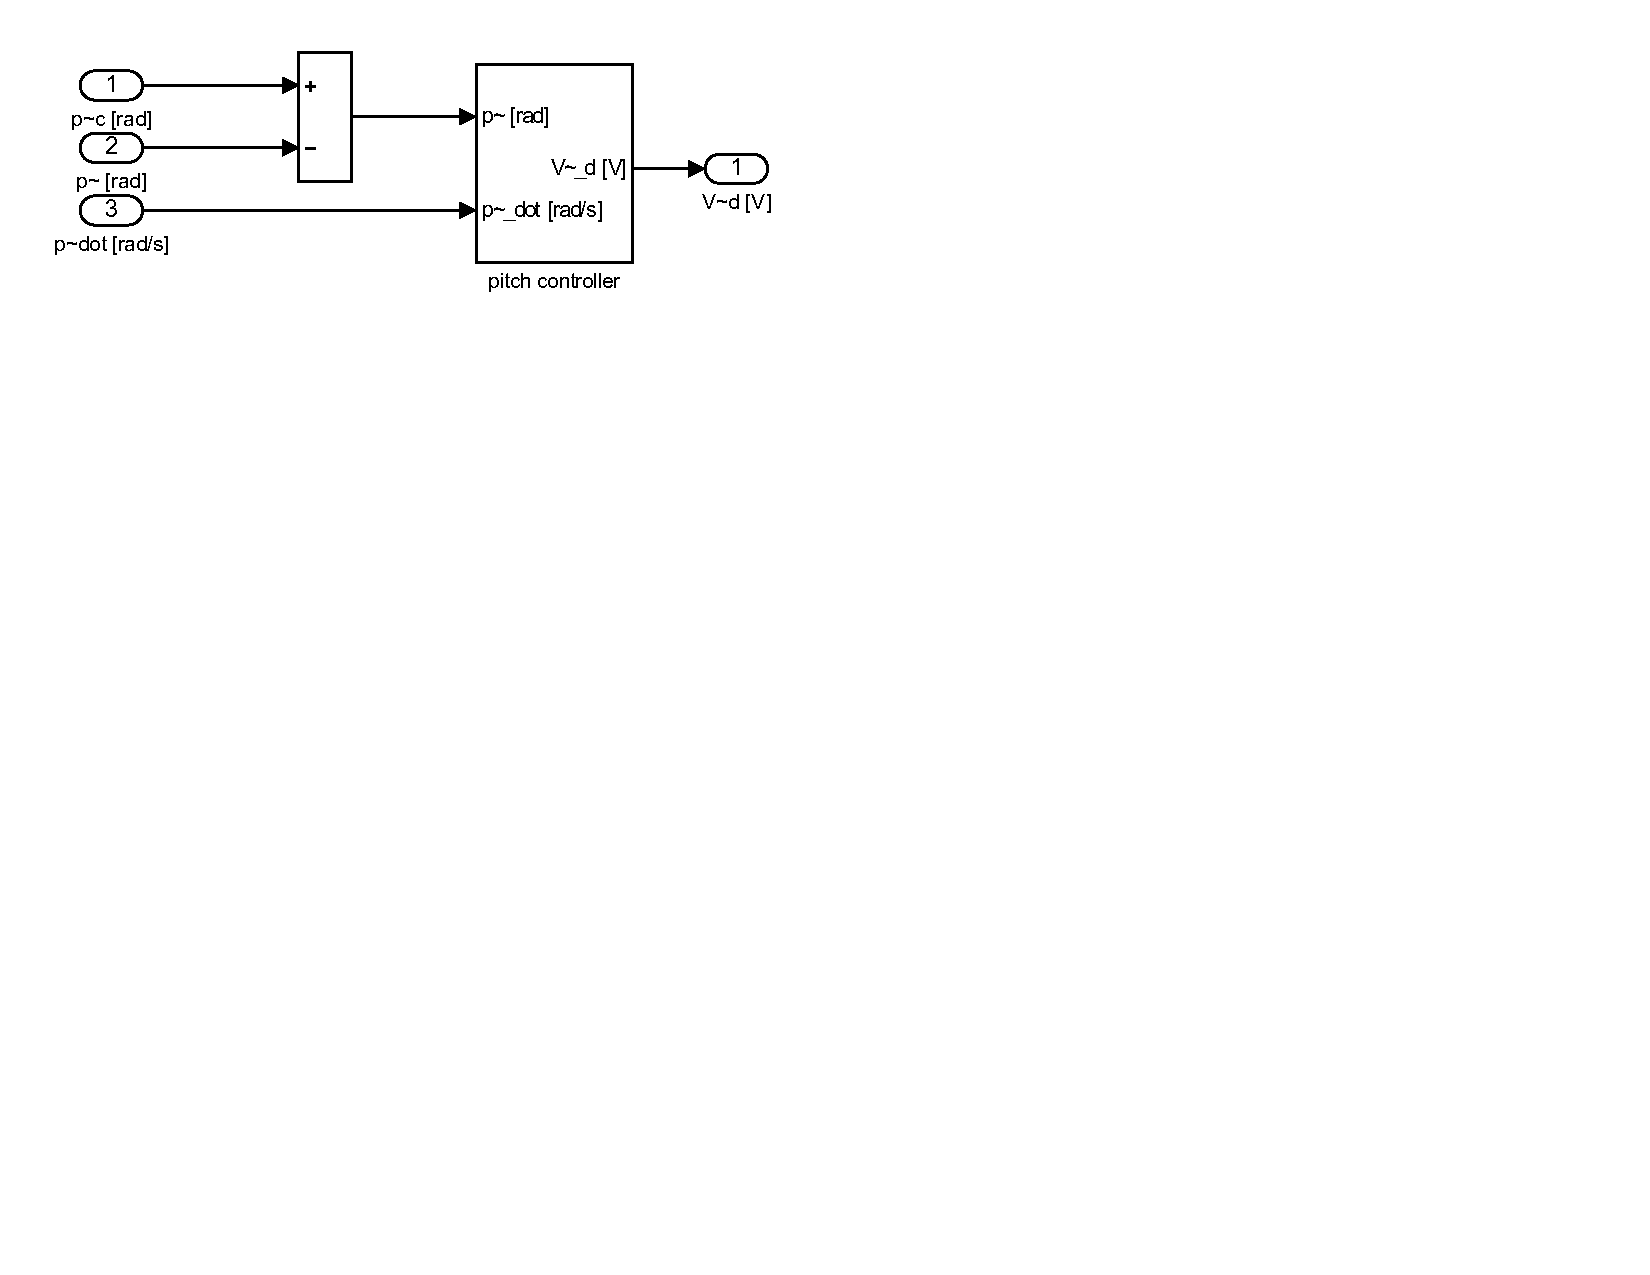
\includegraphics[trim={0 16cm 14cm 0}, clip,width=\linewidth]{images/simulink/P2_pitch.pdf}
	    \caption{Simulink diagram for pitch controller}
        \label{fig:simulink_pitch}
    \end{minipage}\hspace{0.1\textwidth}%
    \begin{minipage}{.45\textwidth}
        \centering
	    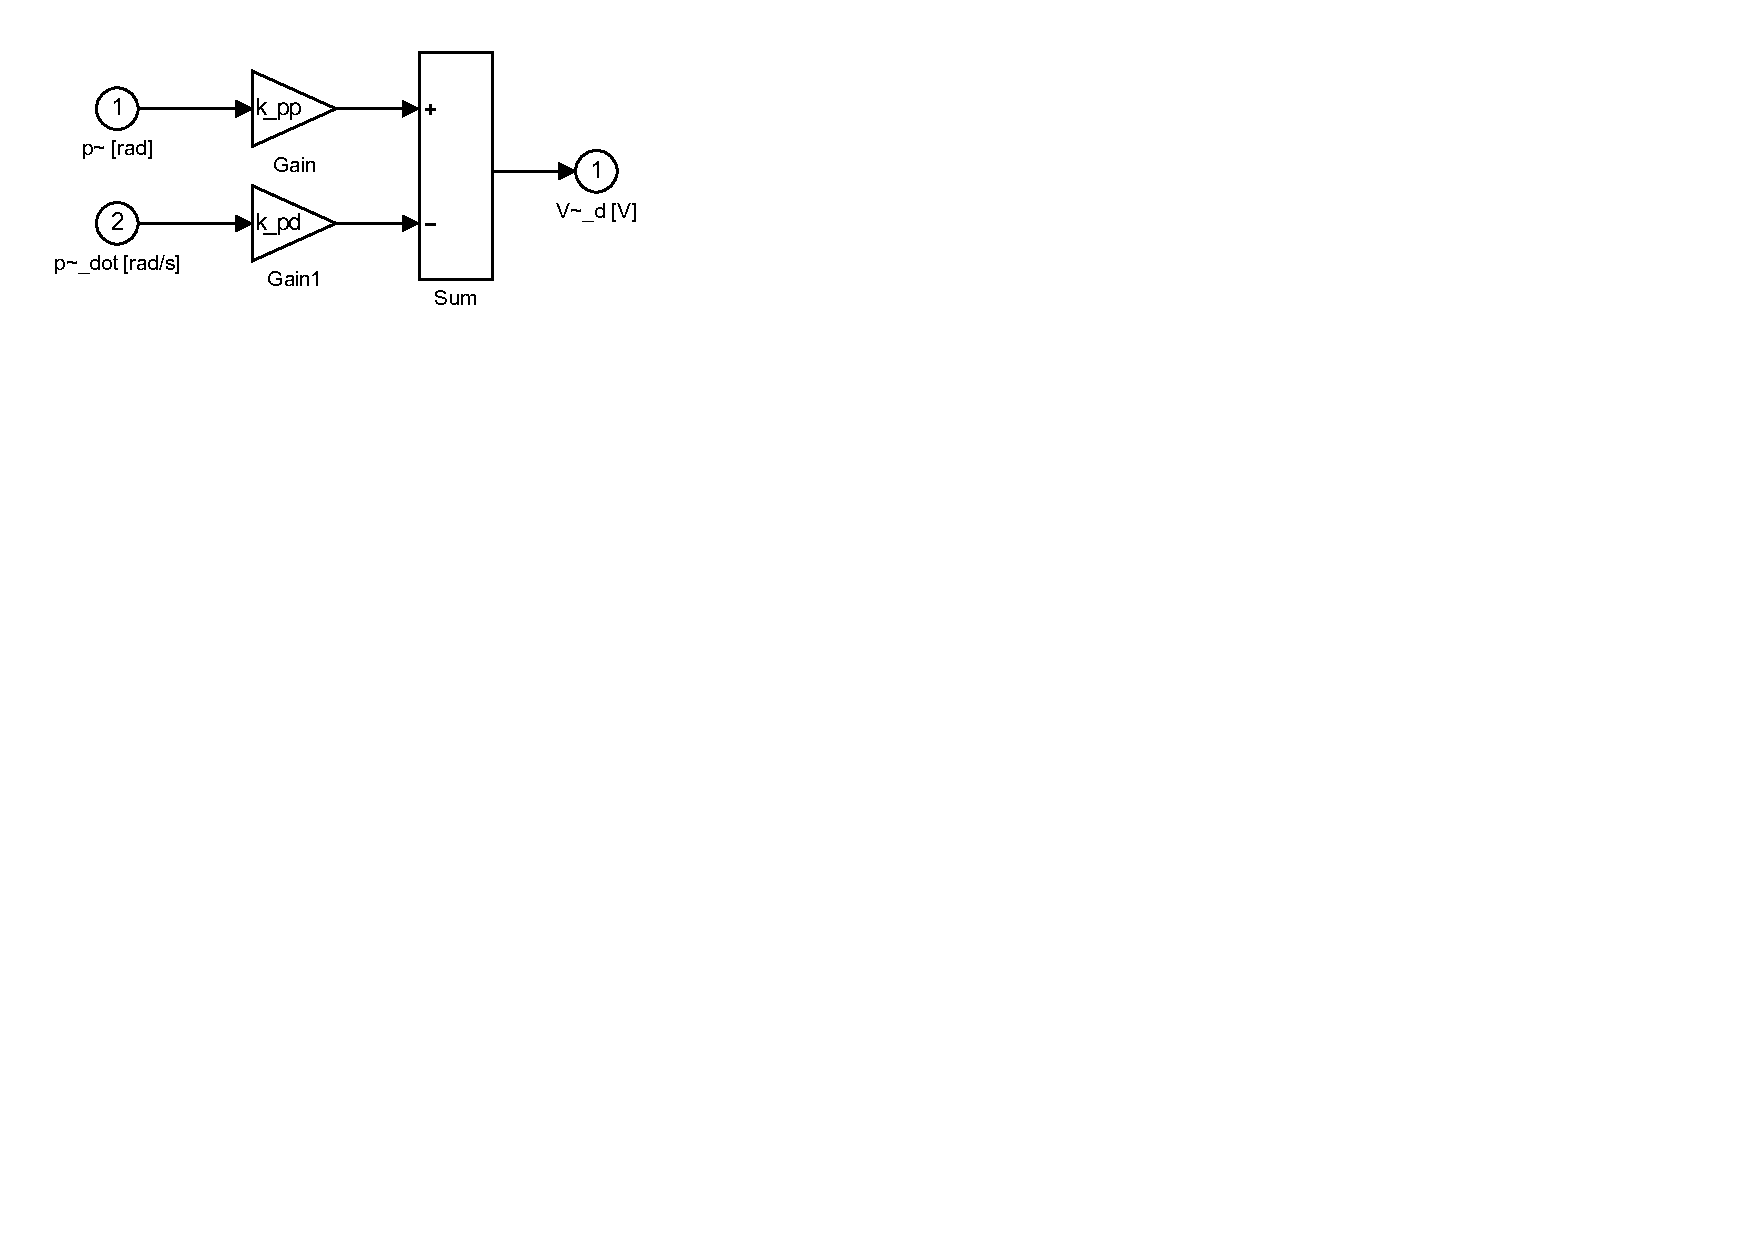
\includegraphics[trim={0 15.5cm 16cm 0}, clip,width=\linewidth]{images/simulink/P2_pitch_controller.pdf}
	    \caption{Simulink diagram for pitch controller subblock}
        \label{fig:simulink_pitch_controller}
    \end{minipage}
    
\end{figure}


By tuning the value of $\omega_0$ in eqs. (\ref{eq:part2_prob2_pd_1}) and (\ref{eq:part2_prob2_pd_2}), we can achieve different responses for the pitch controller.
\medskip

By testing we found the system to be optimally tuned when $\omega_0 = \pi$, this is the value we continued using. The pitch response to step inputs can be seen in Figure \ref{fig:pitch_pi}. To illustrate the response when choosing $\omega_0$ too low or too high, we have included the responses for $\omega_0 = \pi/2$ and $\omega_0 = 2\pi$ 
%and their change rates 
in Figures \ref{fig:pitch_pi_half} to \ref{fig:pitch_2pi}.

\begin{figure}[htb]
	%\centering
	\hspace{-2.7cm}
	\begin{minipage}{.5\textwidth}
	    \centering
		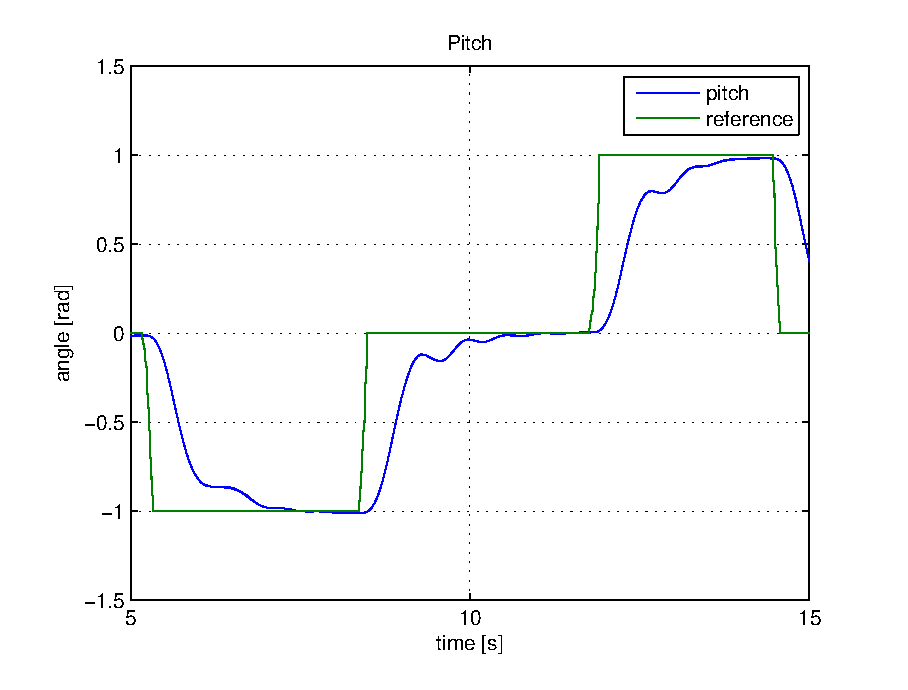
\includegraphics[width=0.9\linewidth]{plots/part2new/pitch_pi.eps}
	    \caption{Pitch with $\omega_0 = \pi$.}
        \label{fig:pitch_pi}
    \end{minipage}%
    \begin{minipage}{.5\textwidth}
        \centering
		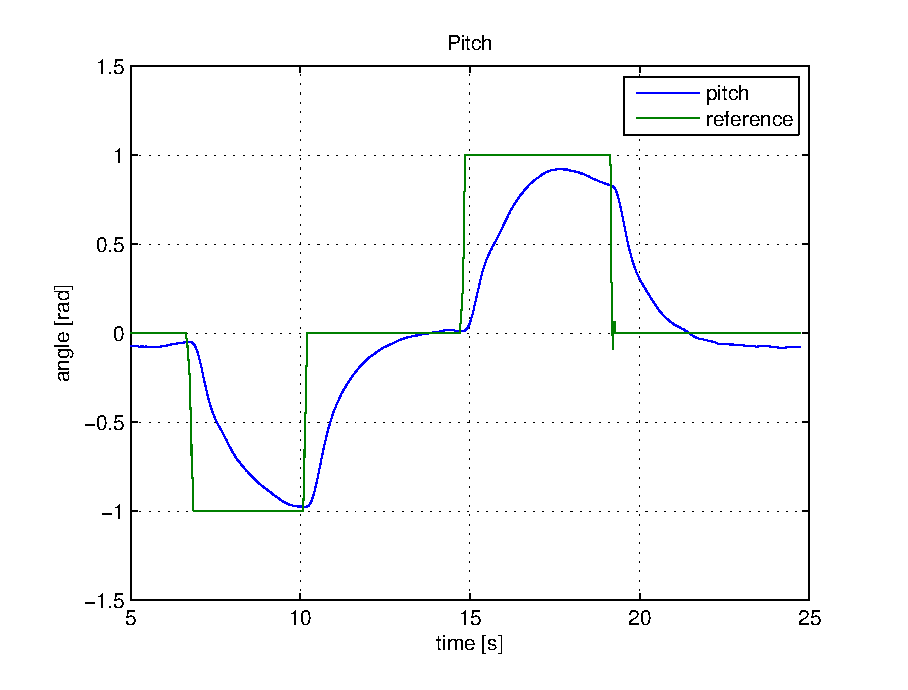
\includegraphics[width=0.9\linewidth]{plots/part2new/pitch_pi_half.eps}
	    \caption{Pitch with $\omega_0 = \pi$/2.}
        \label{fig:pitch_pi_half}
    \end{minipage}%
    \begin{minipage}{.5\textwidth}
    \centering
		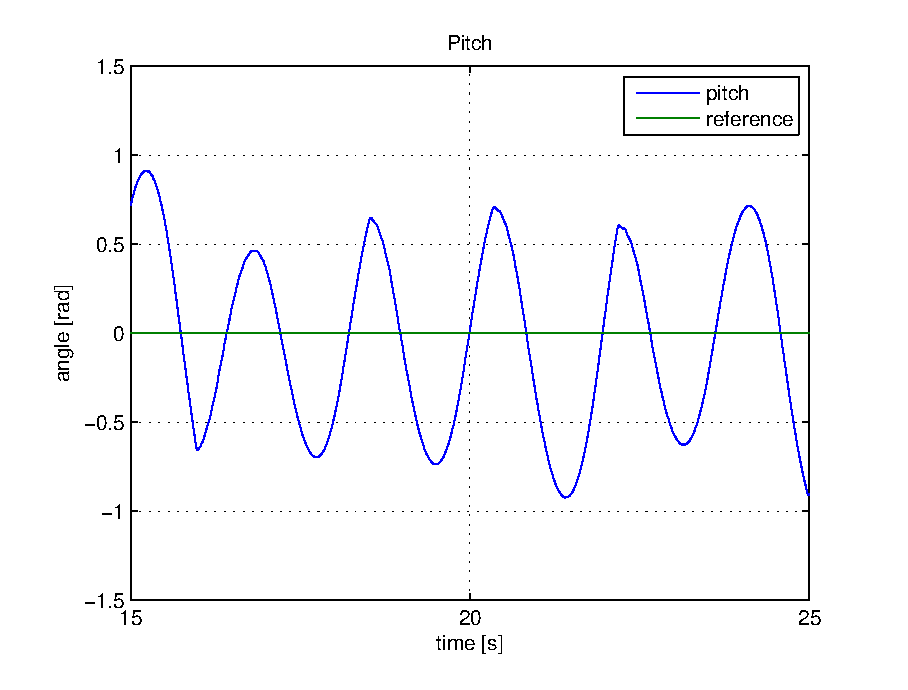
\includegraphics[width=0.9\textwidth]{plots/part2new/pitch_2pi.eps}
	    \caption{Pitch with $\omega_0 = 2 \pi$.}
        \label{fig:pitch_2pi}
    \end{minipage}
    
\end{figure}

%\begin{figure}[htb]
	%\centering
%% 	\hspace{-2.4cm}
%    \begin{minipage}{.5\textwidth}
%	    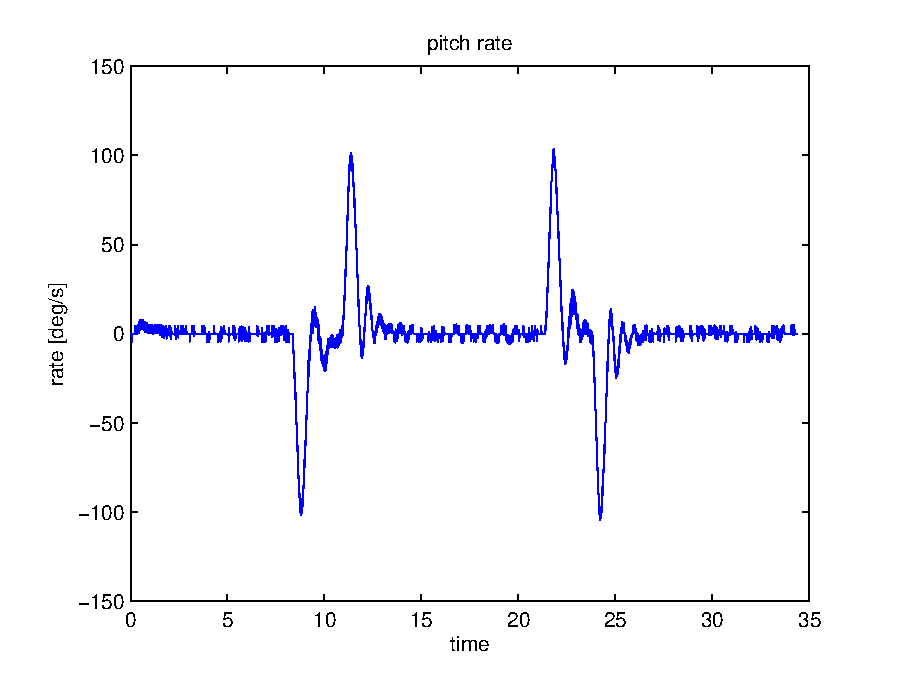
\includegraphics[width=0.9\textwidth]{plots/part2/pitch_rate_pi.eps}
%	    \caption{Pitch rate with $\omega_0 = \pi$.}
%        \label{fig:pitch_rate_pi}
%    \end{minipage}%
%    \begin{minipage}{.5\textwidth}
%        \centering
%		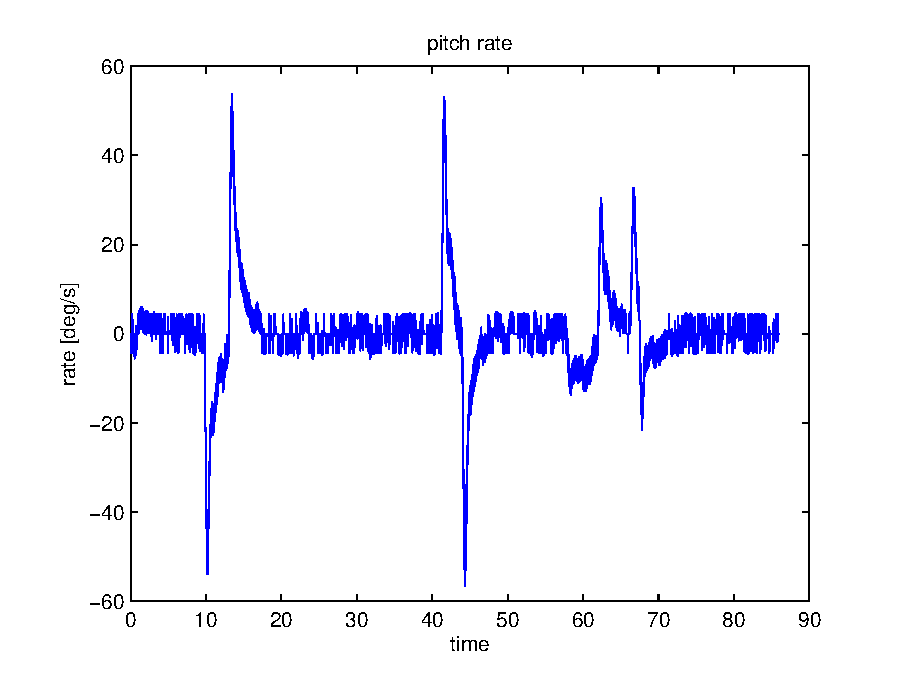
\includegraphics[width=0.9\textwidth]{plots/part2/pitch_rate_pi_half.eps}
%	    \caption{Pitch rate with $\omega_0 = \pi/2$.}
%        \label{fig:pitch_rate_pi_half}
%    \end{minipage}%
%    \begin{minipage}{.5\textwidth}
%    \centering
%		\centering
%		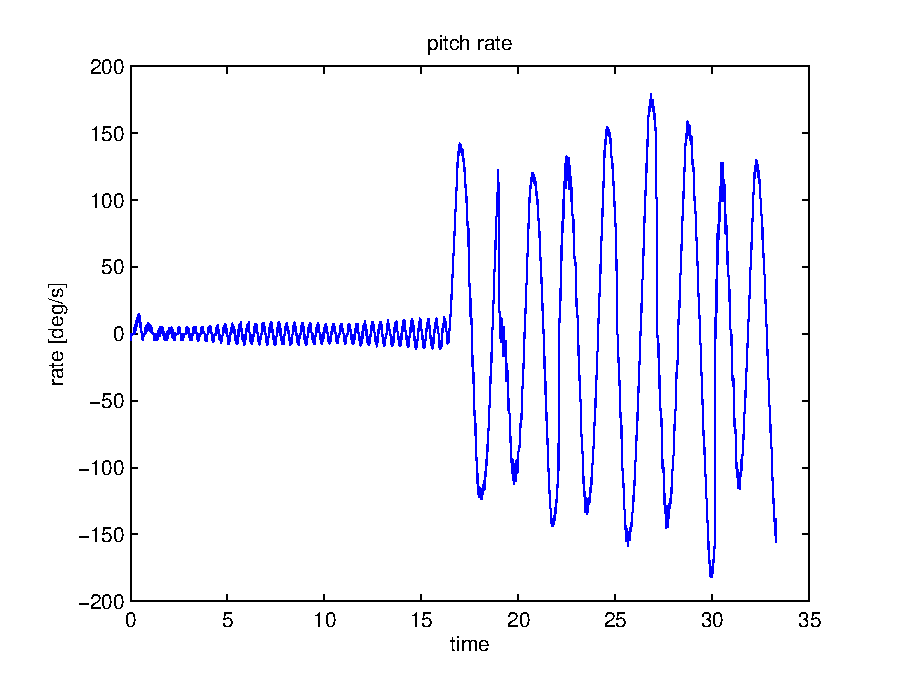
\includegraphics[width=0.9\textwidth]{plots/part2/pitch_rate_2pi.eps}
%	    \caption{Pitch rate with $\omega_0 = 2 \pi$.}
%        \label{fig:pitch_rate_2pi}
%    \end{minipage}
%	
%\end{figure}

As we see, the response is fast an accurate for $\omega_0 = \pi$ in Figures \ref{fig:pitch_pi}. When $\omega_0 = \pi/2$, the pitch angle is slower and does not reach the reference, and as we see from Figure \ref{fig:pitch_pi_half}. $\omega_0 = 2 \pi$ gives unstable oscillations, these would increase if pitch did not have a maximum physical value.
\medskip

By inserting $\omega_0 = \pi$ into eq. (\ref{eq:part2_prob1_K}), we get $K_{pp} = 16.70$ and $K_{pd} = 10.63$.


%%%%%%%%%%%%%%%%%%%%%%%%%%%%%%%%%%%%%%%%%%%%%%%%%%%%%%%%%%%%%%%%%%%%%%%%%%%%%%%%%%%%%%%%%%%%

%%%%                                PART 2 PROBLEM 2

%%%%%%%%%%%%%%%%%%%%%%%%%%%%%%%%%%%%%%%%%%%%%%%%%%%%%%%%%%%%%%%%%%%%%%%%%%%%%%%%%%%%%%%%%%%%
\subsubsection{Problem 2}
We implemented a P controller for travel rate in Simulink as shown in Figure \ref{fig:simulink_travel}.
\begin{figure}[htb]
	\centering
	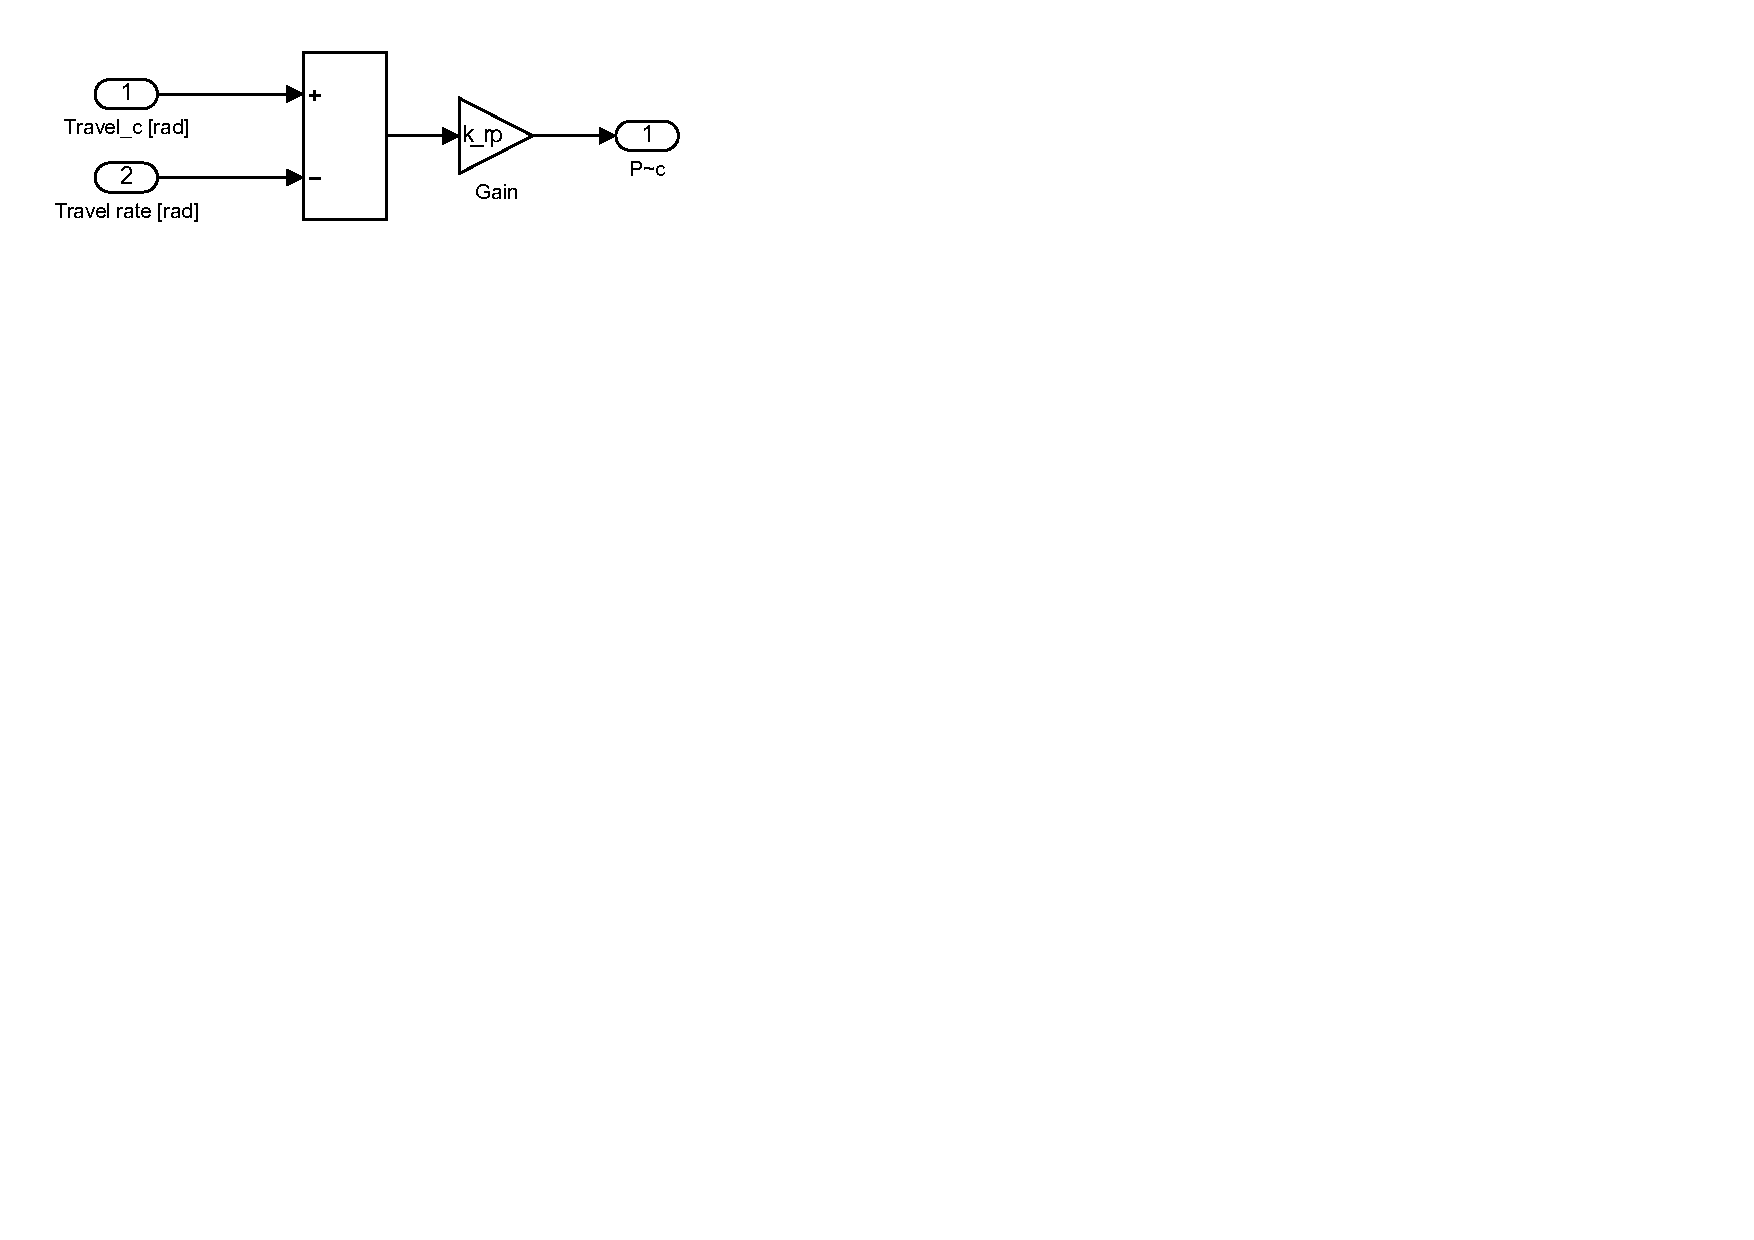
\includegraphics[trim={0 16cm 16cm 0}, clip,width=\linewidth]{images/simulink/P2_travel.pdf}
	\caption{Simulink diagram for travel rate controller}
    \label{fig:simulink_travel}
\end{figure}

We tuned the controller by trying different values of $K_{rp}$ until we found a satisfying response. The plots in Figures \ref{fig:travel_1_1}-\ref{fig:travel_1_5} shows two different choices of $K_{rp}$.
\begin{figure}[htb]
	%\centering
	\hspace{-2.7cm}
	\begin{minipage}{.5\textwidth}
	    \centering
		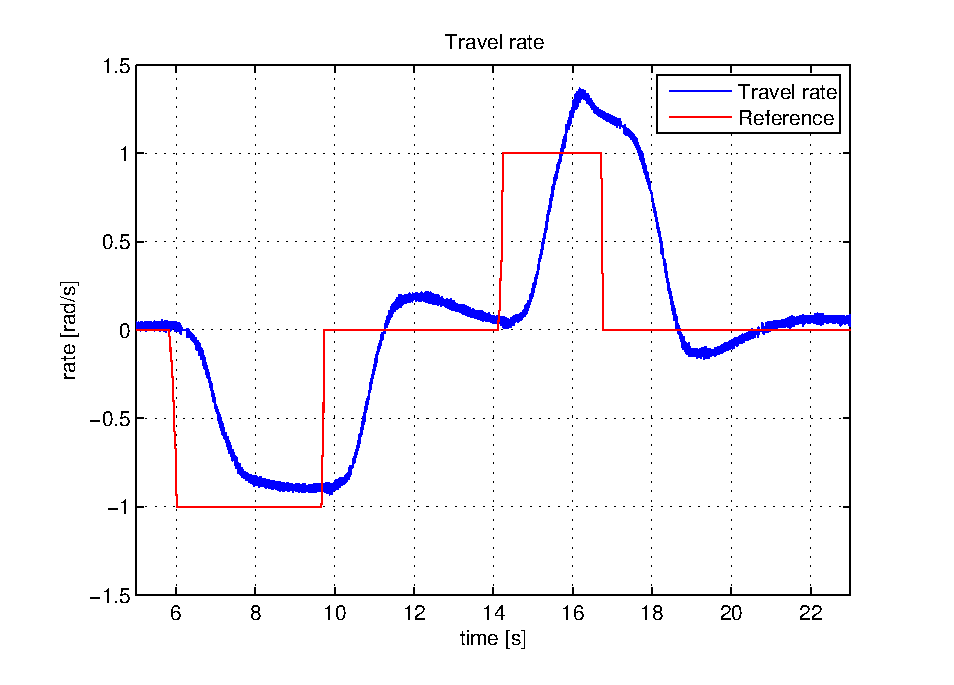
\includegraphics[width=0.9\linewidth]{plots/part2new/travel_rate_1_1.eps}
	    \caption{Travel rate, $K_{rp} = -1.1$.}
        \label{fig:travel_1_1}
    \end{minipage}%
    \begin{minipage}{.5\textwidth}
        \centering
		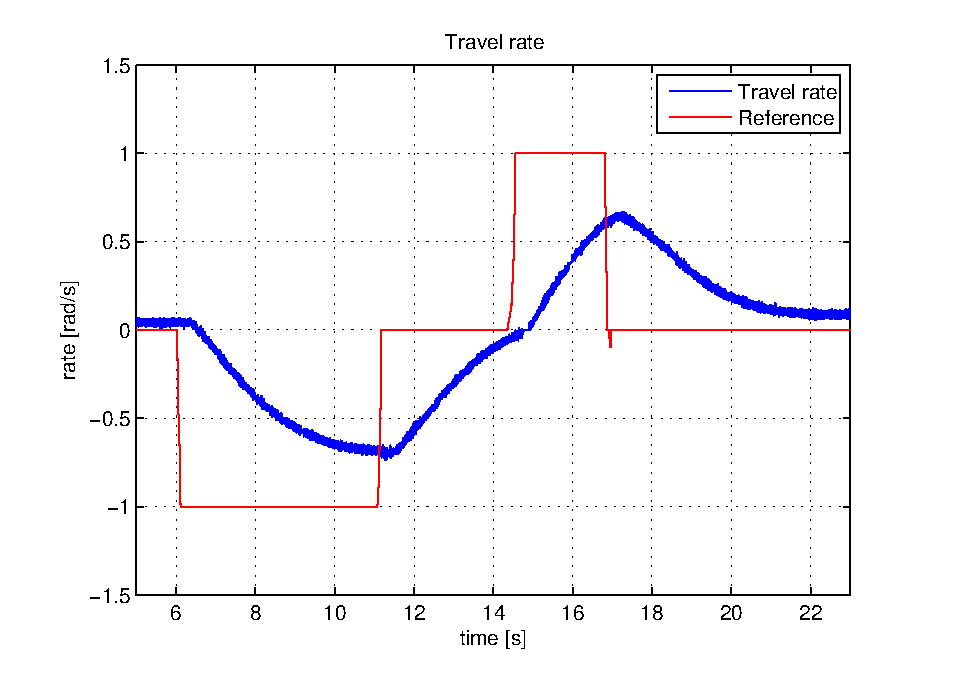
\includegraphics[width=0.9\linewidth]{plots/part2new/travel_rate_0_5.eps}
	    \caption{Travel rate, $K_{rp} = -0.5$.}
        \label{fig:travel_half}
    \end{minipage}%
    \begin{minipage}{.5\textwidth} 
    \centering 
		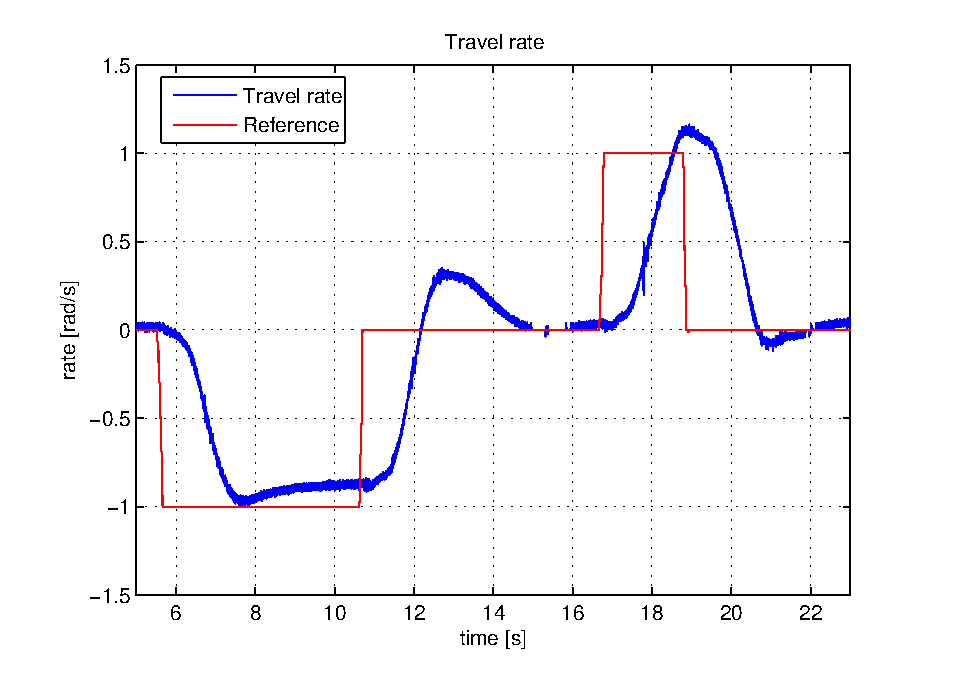
\includegraphics[width=0.9\textwidth]{plots/part2new/travel_rate_1_5.eps}
	    \caption{Travel rate, $K_{rp} = -1.5$.}
        \label{fig:travel_1_5}
    \end{minipage}
    
\end{figure}
Choosing $K_{rp} = -1.1$ gave the faster and more accurate response.


\subsection{Part 3}
\subsubsection{Problem 2}
%%%%%%%%%%%%%%%%%%%%%%%%%%%%%%%%%%%%%%%%%%%%%%%%%%%%%%%%%%%%%%%%%%%%%%%%%%%%%%%%%%%%%%%%%%%%

%%%%                                PART 3 PROBLEM 2

%%%%%%%%%%%%%%%%%%%%%%%%%%%%%%%%%%%%%%%%%%%%%%%%%%%%%%%%%%%%%%%%%%%%%%%%%%%%%%%%%%%%%%%%%%%%

We now add an LQR controller to our system, aiming to control the pitch angle and elevation rate. The controller is given by eq. (\ref{eq:part3_prob2_state_feedback}). The Simulink diagram can be seen in Figure \ref{fig:simulink_multivariabe}.\medskip

\begin{figure}[h!]
	\centering
	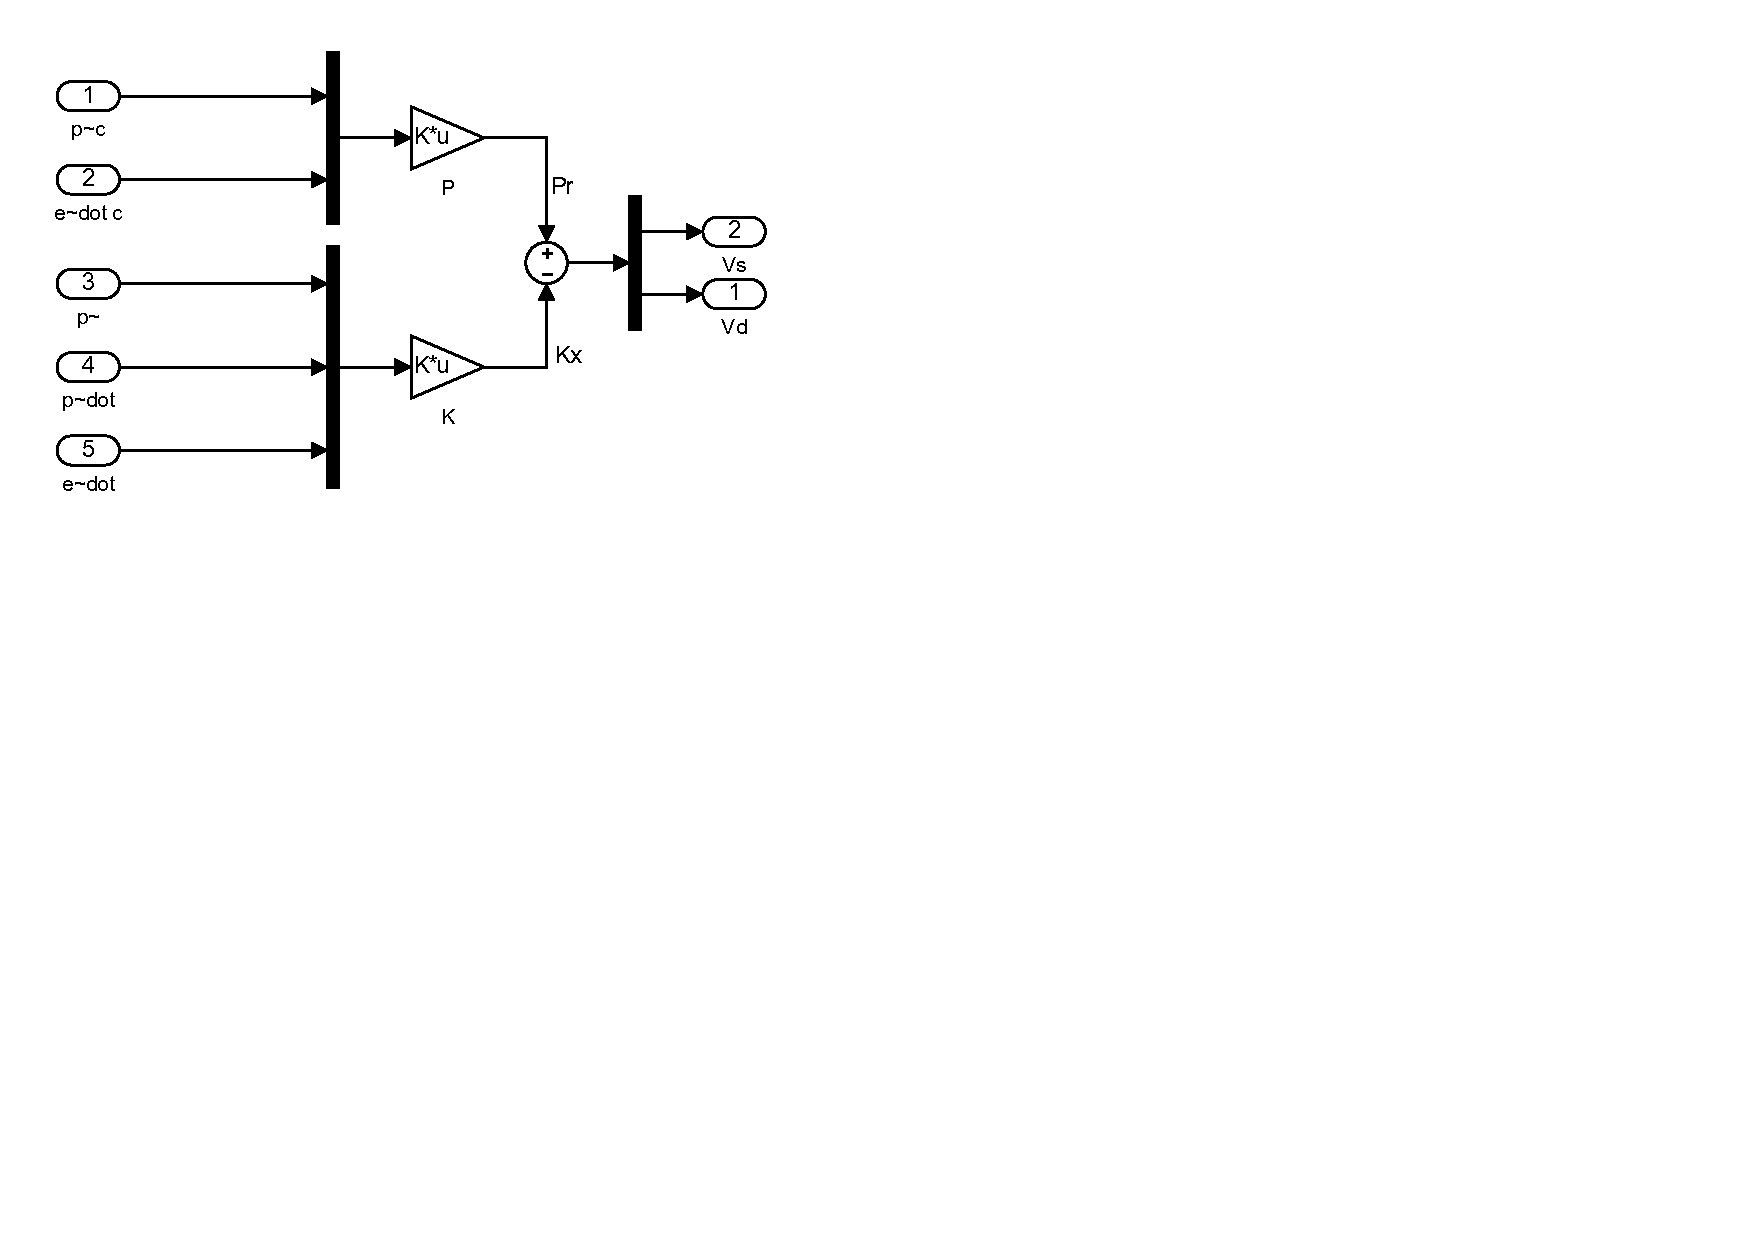
\includegraphics[scale=0.8, trim={0 12cm 16cm 0}, clip]{images/simulink/P3.pdf}
	\caption{Simulink diagram for multivariable controller}
    \label{fig:simulink_multivariabe}
\end{figure}


When tuning the weighting matrices \textbf{Q} and \textbf{R} we have to  keep the system as close to the linearized model as possible or the assumptions made in (\ref{eq:state_space}) will no longer be valid. We started with $1$ on all the values. We want to control pitch and elevation rate, so these values were increased if the system was to slow/far away from the references. When the system would overshoot, we increased the value in $R$, so that the regulator can't use as much input, and lowered them when they failed to reach the reference. After repeating these steps a few times we found our final values. The final weighting matrices are seen in (\ref{eq:Q_p}) and (\ref{eq:R_p}). 

\begin{equation} \label{eq:Q_p}
    \bm{Q} = 
	\begin{bmatrix}
		10000 & 0     & 0\\
		0     & 10    & 0\\
		0     & 0     & 100000\\
	\end{bmatrix}
\end{equation} 

\begin{equation} \label{eq:R_p}
    \bm{R} = 
	\begin{bmatrix}
		100   & 0  \\
		0     & 100\\
	\end{bmatrix}
\end{equation} 

With these weighting matrices, $\bm{K}$ and $\bm{P}$ become
\begin{equation} \label{eq:K_p}
    \bm{K} = 
	\begin{bmatrix}
		0     & 0     & 31.62\\
		10    & 5.828 & 0    \\
	\end{bmatrix}
\end{equation} 

\begin{equation} \label{eq:P_p}
    \bm{P} = 
	\begin{bmatrix}
		0     & 31.62\\
		10    & 0    \\
	\end{bmatrix}
\end{equation} 

The resulting responses for elevation rate and pitch angle can be seen in Figure \ref{fig:Elevationrate_p} and \ref{fig:Pitch_p}.

\begin{figure}[h!]
	%\centering
 	%\hspace{-2.4cm}
    \begin{minipage}{.45\textwidth}
	    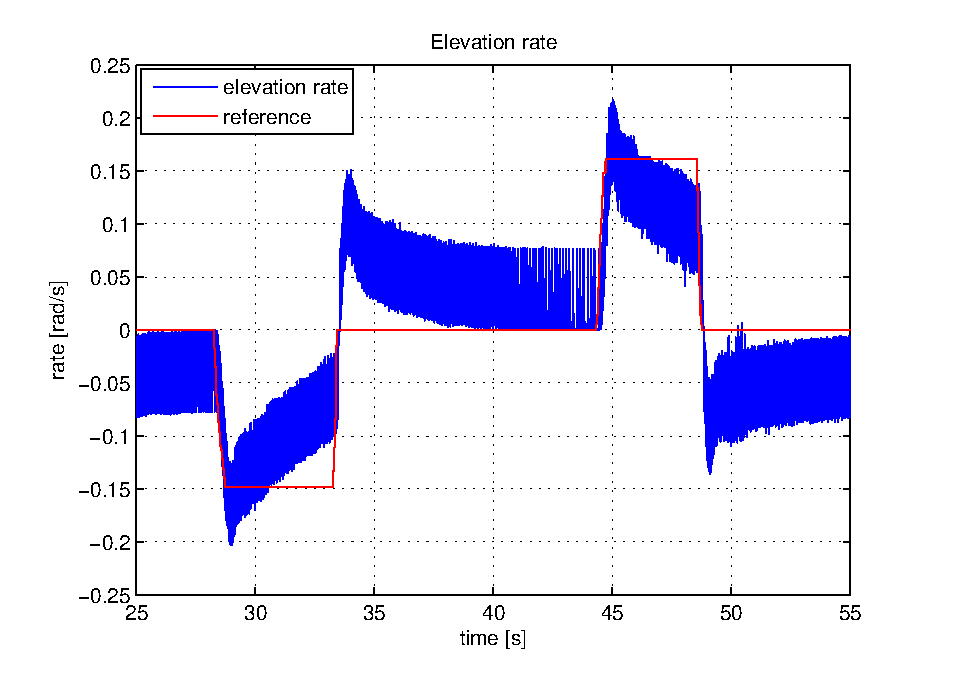
\includegraphics[width=1\textwidth]{plots/part3/part2/Elevationrate.eps}
	    \caption{Elevation rate with LQR.}
        \label{fig:Elevationrate_p}
    \end{minipage}\hspace{0.1\textwidth}%
    \begin{minipage}{.45\textwidth}
        \centering
		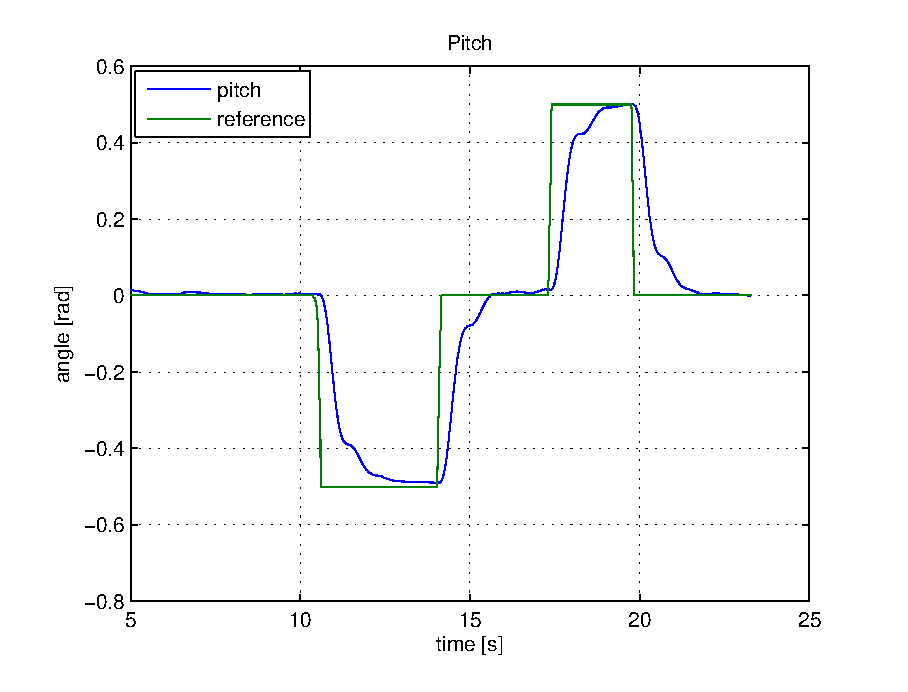
\includegraphics[width=1\textwidth]{plots/part3/part2/Pitch.eps}
	    \caption{Pitch with LQR.}
        \label{fig:Pitch_p}
    \end{minipage}
\end{figure}
\medskip

From Figure \ref{fig:Elevationrate_p} we can see that the LQR controller alone is not enough to control the elevation rate. This is a result of having a linearized model. As the helicopter moves away from the zero state the nonlinearity in (\ref{eq:model_se_al_elev}) forces the helicopter back to its zero state. 

%%%%%%%%%%%%%%%%%%%%%%%%%%%%%%%%%%%%%%%%%%%%%%%%%%%%%%%%%%%%%%%%%%%%%%%%%%%%%%%%%%%%%%%%%%%%

%%%%                                PART 3 PROBLEM 3

%%%%%%%%%%%%%%%%%%%%%%%%%%%%%%%%%%%%%%%%%%%%%%%%%%%%%%%%%%%%%%%%%%%%%%%%%%%%%%%%%%%%%%%%%%%%
\subsubsection{Problem 3}
We wanted to include the integral effect to mitigate the effects of linearizing the model, this is most significant for $\dot{\tilde{e}}$. This works by integrating the steady state error that occurs from the change of gravitational force on the helicopter when it moves away from the zero state. In effect this will set a reference elevation that the the system til try to return to, even when exposed to external physical disturbances. 
\medskip

The Simulink model for the multivariable controller with integral effect can be seen in Figure \ref{fig:simulink_multivariable_integral}.

\begin{figure}[h]
	\centering
	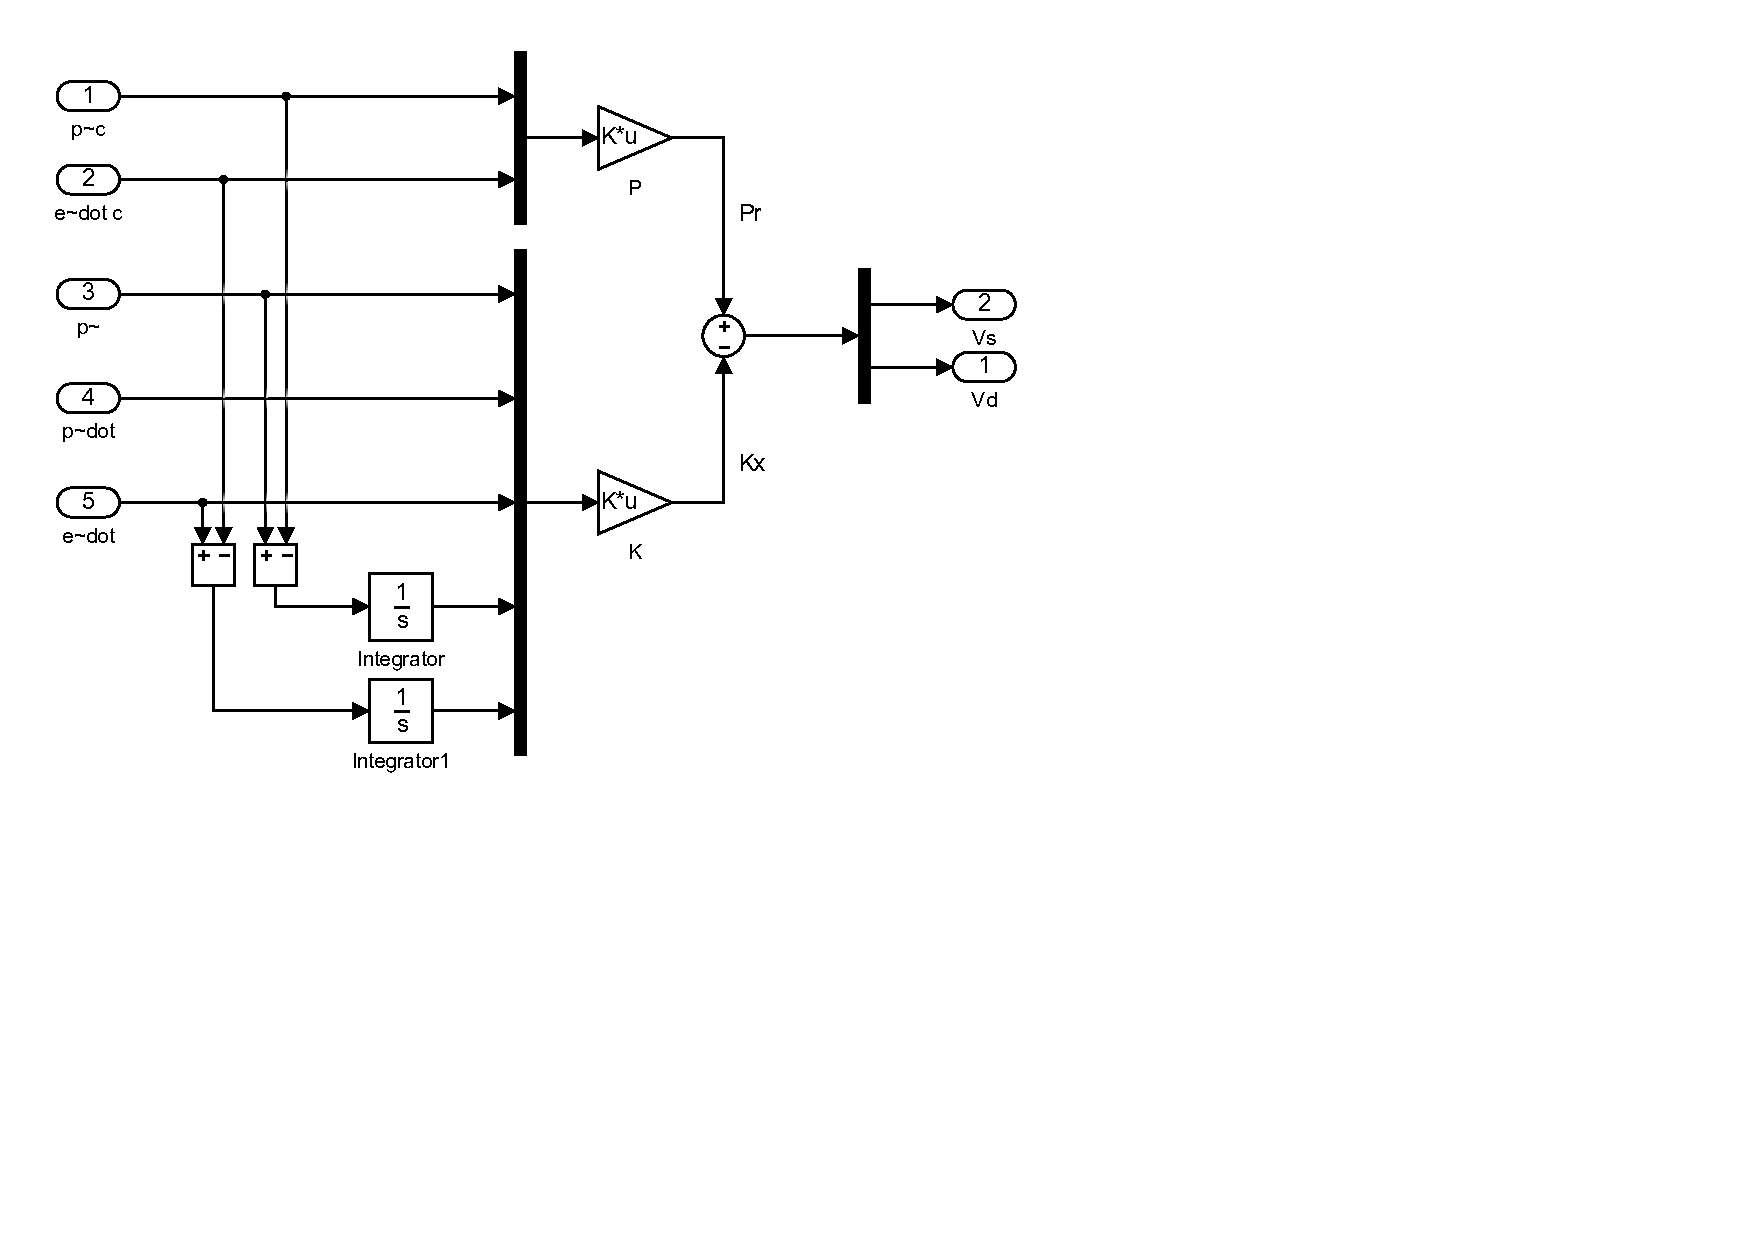
\includegraphics[trim={0 7cm 12cm 0}, clip,scale=0.6]{images/simulink/P3_integral.pdf}
	\caption{Simulink diagram for multivariable controller with integral effect.}
    \label{fig:simulink_multivariable_integral}
\end{figure}

\medskip

When deciding how to weight $\dot{\gamma}$ and $\dot{\zeta}$ we knew that the pitch using the LQR controller already gave us good results, while the elevation rate would be more dependant on the integral effect. We therefore weighted $\dot{\gamma}$ lower than $\dot{\zeta}$ which we weigh quite high. After tuning the controller the final values for $\bm{Q}_i$ and $\bm{R}_i$ are

\begin{equation} \label{eq:Q_pi}
    \bm{Q}_i = 
	\begin{bmatrix}
		10000 &  0    &  0      &  0   &  0 \\
		0     &  10   &  0      &  0   &  0 \\
		0     &  0    &  10000  &  0   &  0 \\
		0     &  0    &  0      &  100 &  0 \\
		0     &  0    &  0      &  0   &  10000
	\end{bmatrix}
\end{equation} 

\begin{equation} \label{eq:R_pi}
    \bm{R}_i = 
	\begin{bmatrix}
		75   & 0  \\
		0    & 100\\

	\end{bmatrix}
\end{equation} 

After optimizing the cost function (\ref{eq:cost_function}) using the matlab command \texttt{lqr(A, B, Q, R)} - where \texttt{A}, \texttt{B}, \texttt{Q} and \texttt{R} are  respectively $\bm{A}_i$, $\bm{B}_i$, $\bm{Q}_i$ and $\bm{R}_i$,
we acquire the following $\bm{K}_i$ matrix

\begin{equation} \label{eq:K_pi}
    \bm{K}_i = 
	\begin{bmatrix}
		0      &  0      & 17.62 &  0     &  10 \\
		12.04  &  7.13   & 0     &  3.16  &  0 \\
	\end{bmatrix}
\end{equation} 

The resulting response can be seen in Figure \ref{fig:Elevationrate_pi} and \ref{fig:Pitch_p_integral}.
\begin{figure}[h!]
	%\centering
 	%\hspace{-2.4cm}
    \begin{minipage}{.45\textwidth}
	    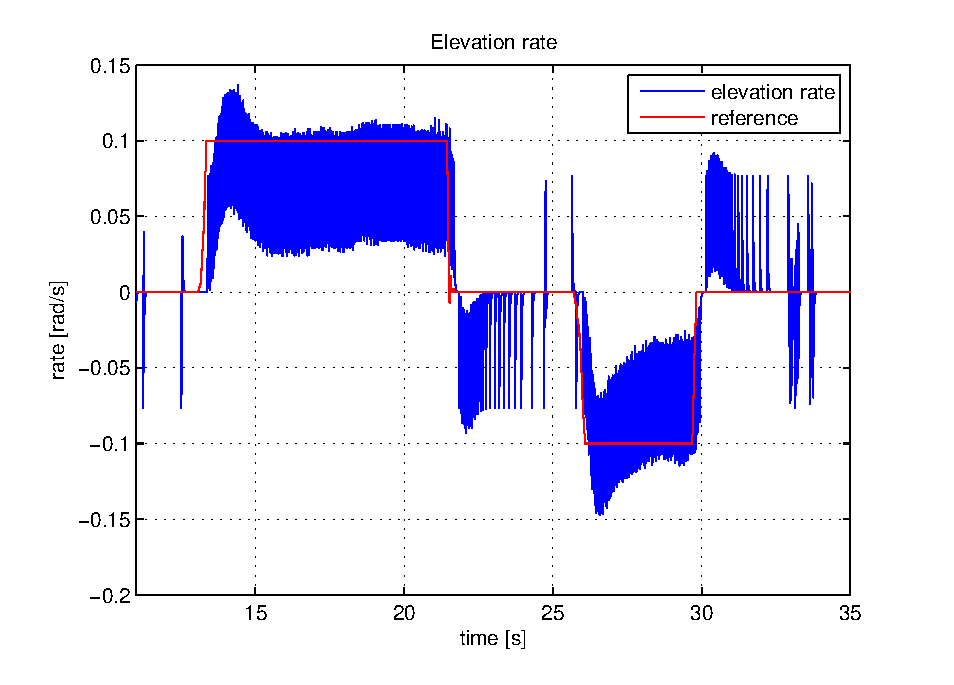
\includegraphics[width=1\textwidth]{plots/part3/part3_integral/elevationrate.eps}
	    \caption{Elevation rate with LQR and integral effect.}
        \label{fig:Elevationrate_pi}
    \end{minipage}\hspace{0.1\textwidth}%
    \begin{minipage}{.45\textwidth}
        \centering
		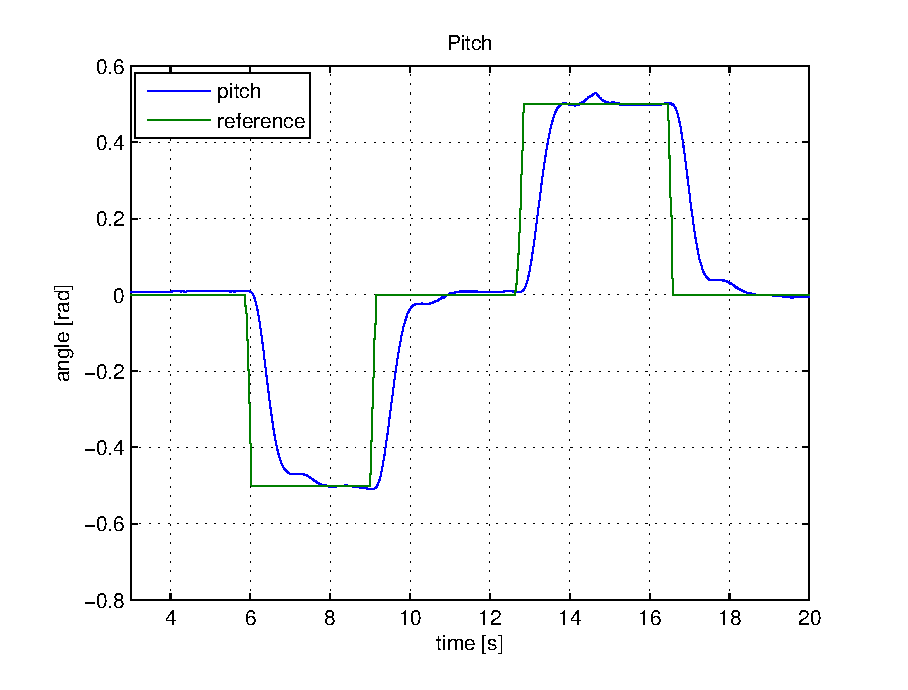
\includegraphics[width=1\textwidth]{plots/part3/part3_integral/pitch.eps}
	    \caption{Pitch with LQR and integral effect.}
        \label{fig:Pitch_p_integral}
    \end{minipage}
\end{figure}
As we see, the elevation rate does not go back to zero as it did with just the LQR in Figure \ref{fig:Elevationrate_p}. The pitch angle in Figure \ref{fig:Pitch_p_integral} is still fast and accurate, the response is about the same as we saw with LQR in Figure \ref{fig:Pitch_p}.

\subsection{Part 4}
%%%%%%%%%%%%%%%%%%%%%%%%%%%%%%%%%%%%%%%%%%%%%%%%%%%%%%%%%%%%%%%%%%%%%%%%%%%%%%%%%%%%%%%%%%%%

%%%%                                PART 4 PROBLEM 1

%%%%%%%%%%%%%%%%%%%%%%%%%%%%%%%%%%%%%%%%%%%%%%%%%%%%%%%%%%%%%%%%%%%%%%%%%%%%%%%%%%%%%%%%%%%%
\subsubsection{Problem 1}
Implemented our new model in Simulink. 
\begin{figure}[h!]
    \centering
	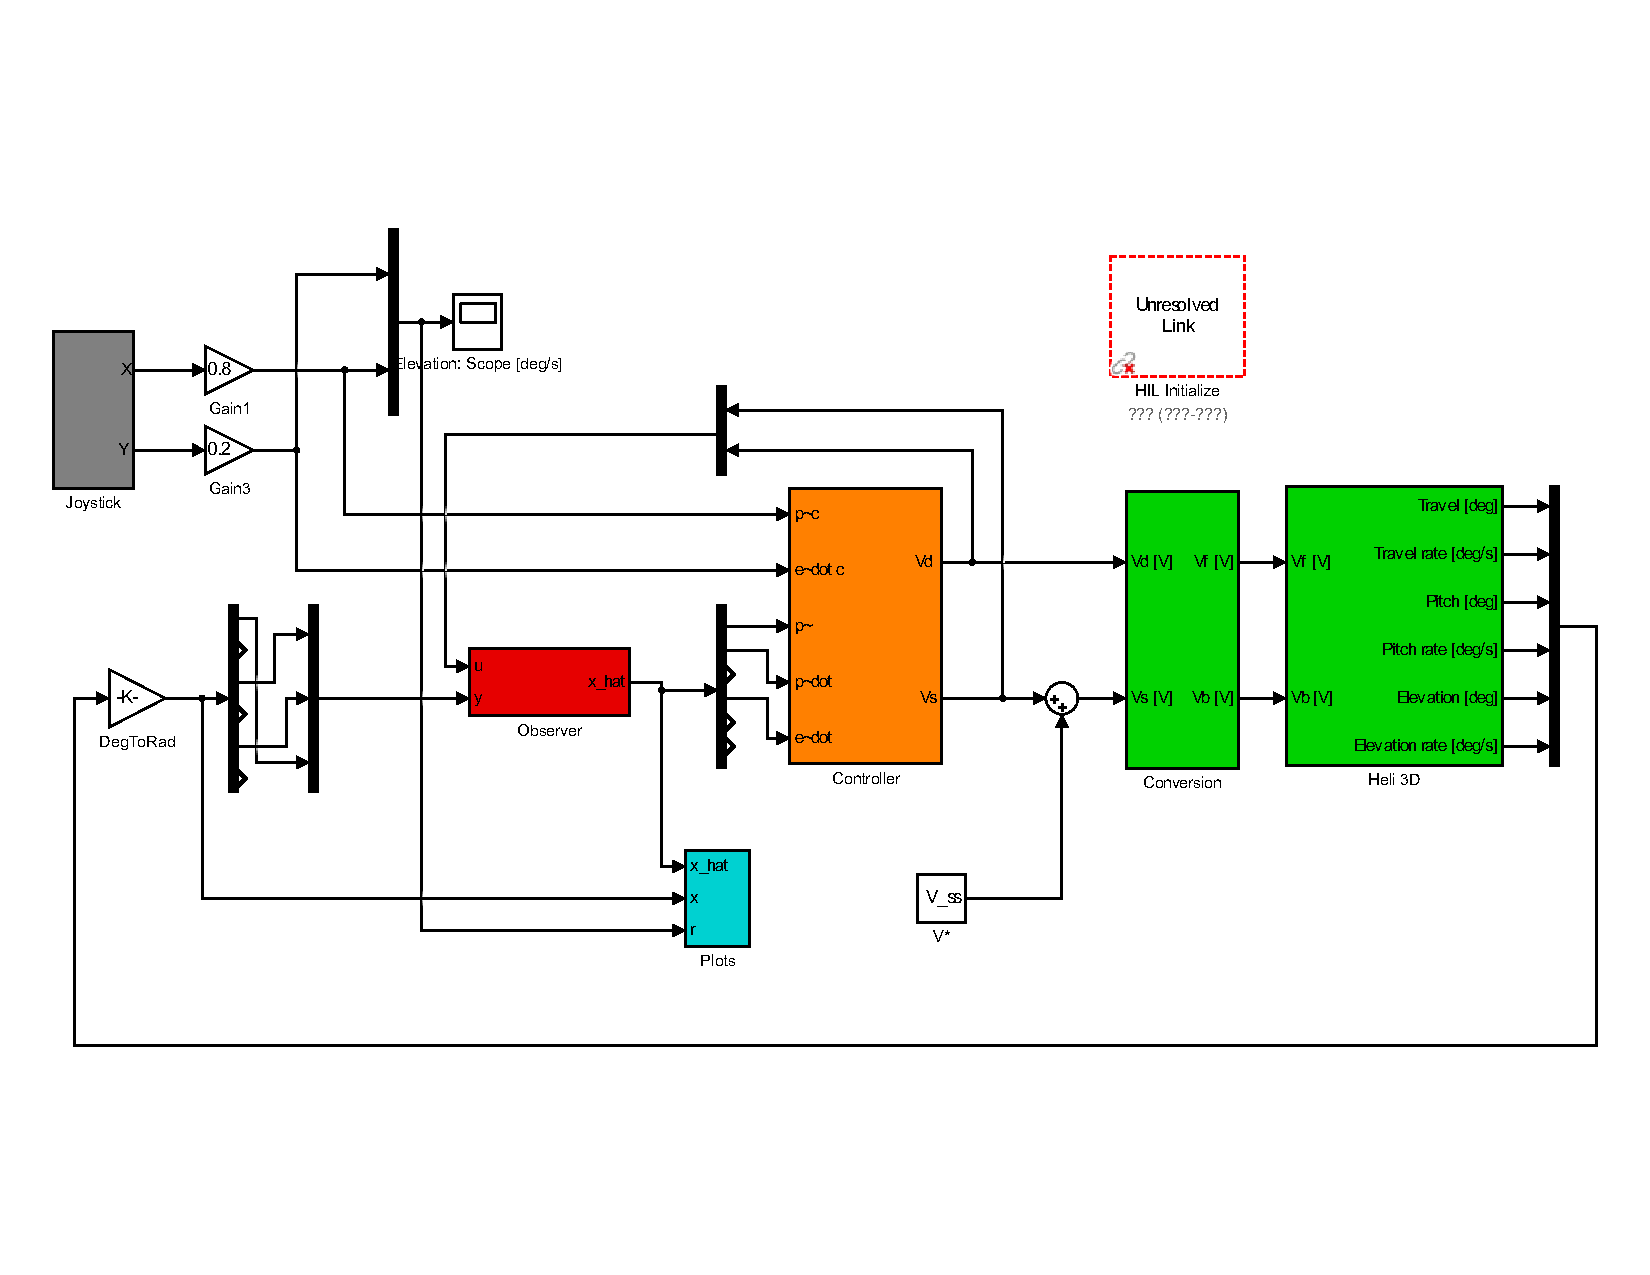
\includegraphics[trim={0 3cm 0 3cm},clip,width=\linewidth]{images/simulink/P4_diag.pdf}
    \caption{Simulink model with observer subsystem}
    \label{fig:simulink_P4}
\end{figure}

\begin{figure}[H]
    \centering
	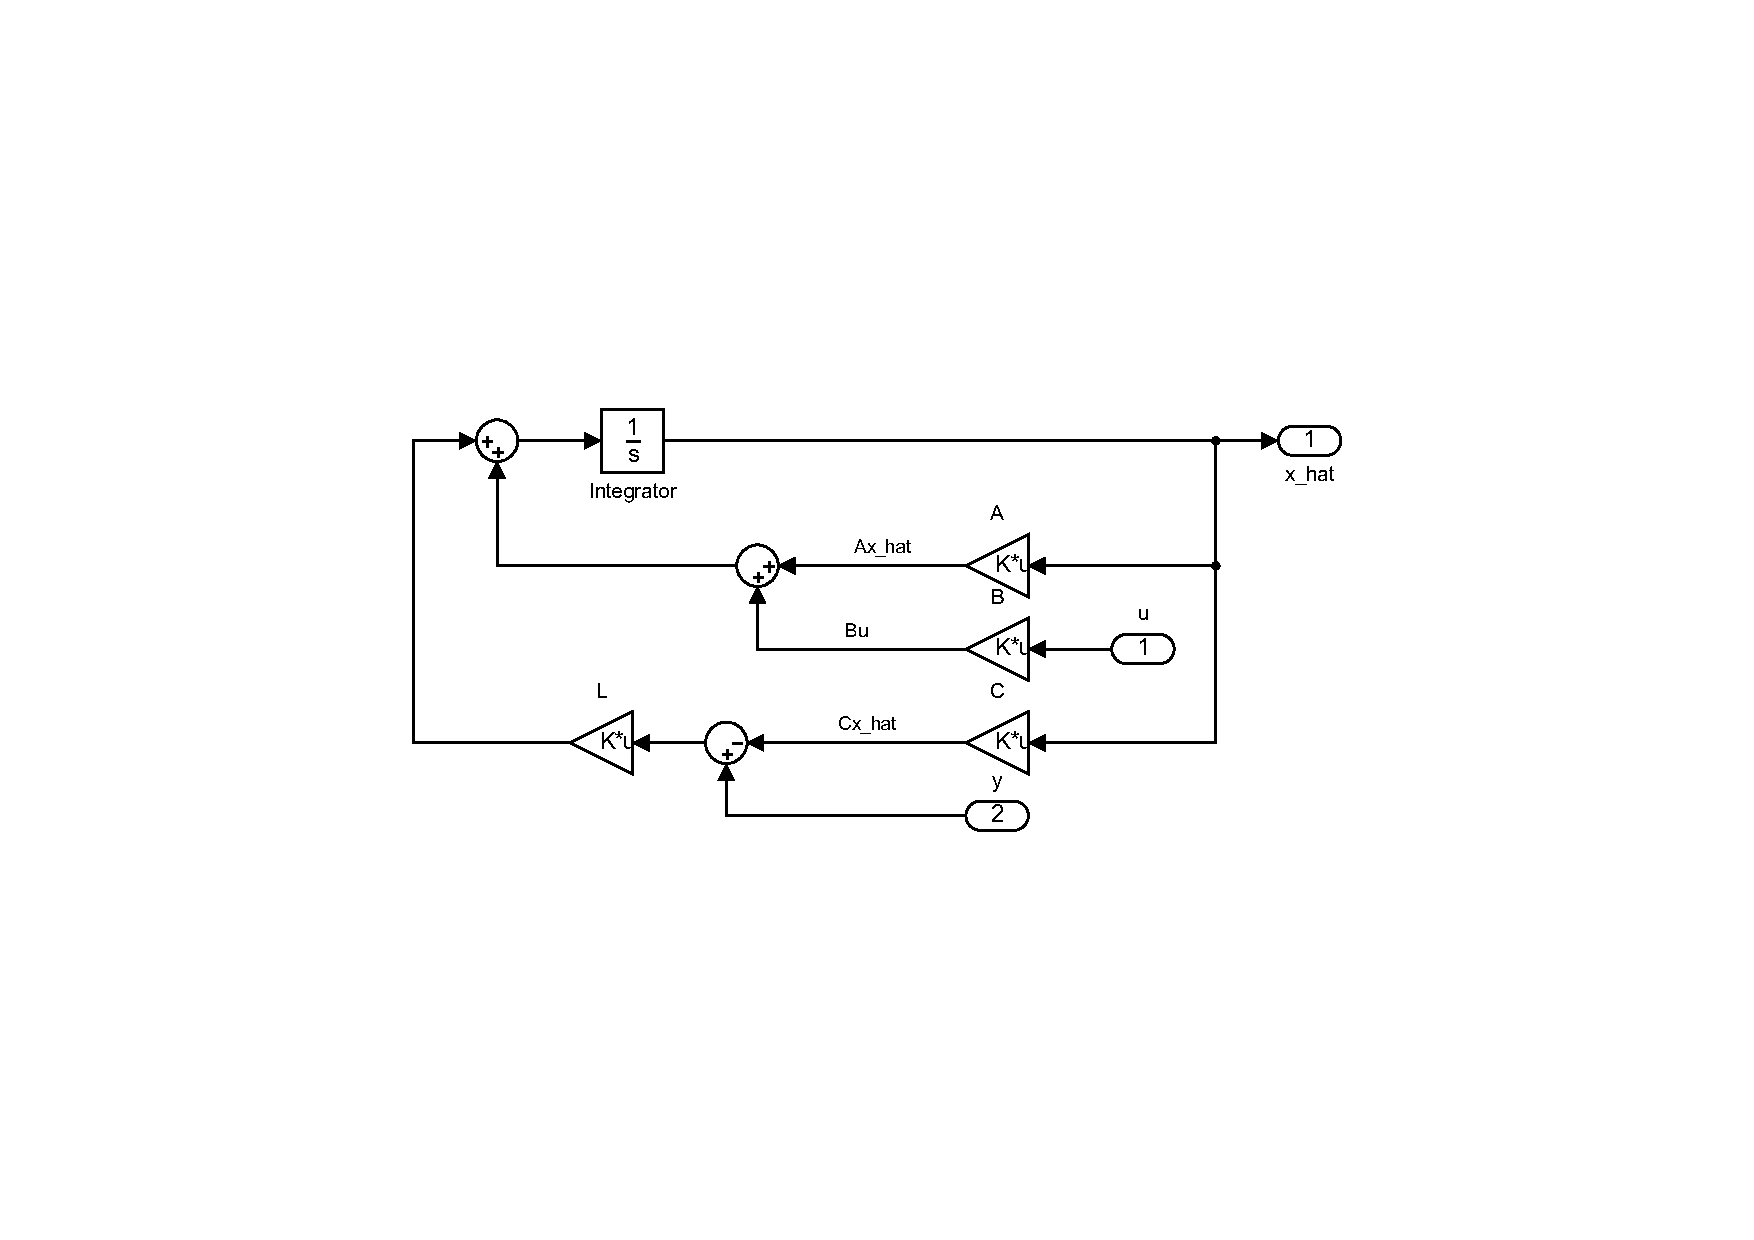
\includegraphics[trim={6.5cm 6.5cm 6.5cm 6.5cm},clip,width=\linewidth]{images/simulink/P4_observer.pdf}
    \caption{Simulink model of observer}
    \label{fig:simulink_P4_observer}
\end{figure}

The estimator is used as input to the controller, instead of the actual measurements $y$. To calculate the estimator, the matrices from the linearized system have been used. This means that the estimator, just like our modelled system, works best when close to the equilibrium. When the system moved away from this point, both the system and the estimator will differ from the real world, meaning that the regulator won't be able to fully regulate the system to the reference. 

%%%%%%%%%%%%%%%%%%%%%%%%%%%%%%%%%%%%%%%%%%%%%%%%%%%%%%%%%%%%%%%%%%%%%%%%%%%%%%%%%%%%%%%%%%%%

%%%%                                PART 4 PROBLEM 2

%%%%%%%%%%%%%%%%%%%%%%%%%%%%%%%%%%%%%%%%%%%%%%%%%%%%%%%%%%%%%%%%%%%%%%%%%%%%%%%%%%%%%%%%%%%%
\subsubsection{Problem 2}
The estimator poles need to be placed in such a way that the estimator will be able to predict the error faster than the system. This means putting the estimator poles further out into the left plane. We used \texttt{r = 10*max(abs(eig(A-BK)))} which gave us an $r = 24$ as a base for our tuning, and adjusted the r value until the estimator followed the actual system without a lot of noice. Matlab code for computing the poles can be found in appendix \ref{sec:matlab_pole_placement}. Some example responses for different values of r can be seen in Figures \ref{fig:e_rate_5}, \ref{fig:e_rate_27} and \ref{fig:e_rate_60}.\\

\begin{figure}[H]
	%\centering
	\hspace{-2.7cm}
	\begin{minipage}{.5\textwidth}
	    \centering
		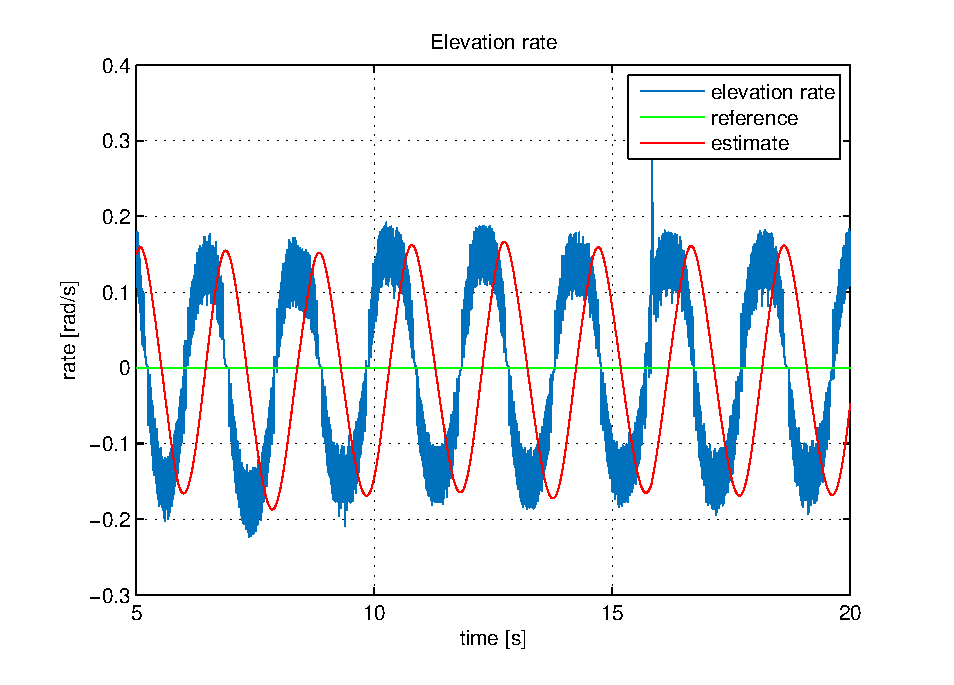
\includegraphics[width=0.9\linewidth]{plots/part4new/P/e_rate_5.eps}
	    \caption{Elevation rate with r = 5.}
        \label{fig:e_rate_5}
    \end{minipage}%
    \begin{minipage}{.5\textwidth}
        \centering
		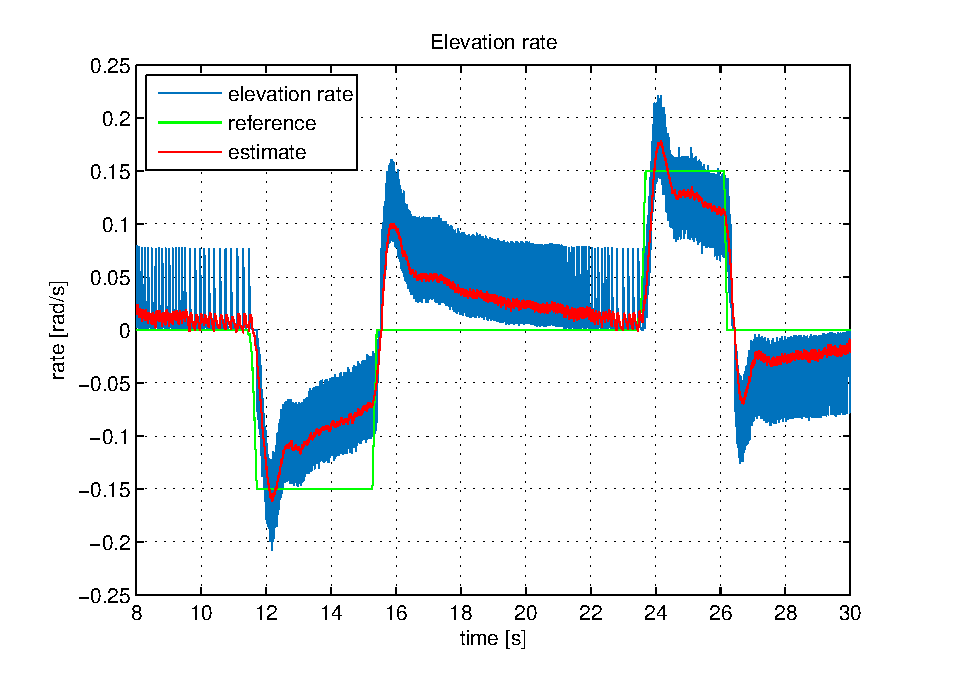
\includegraphics[width=0.9\linewidth]{plots/part4new/P/e_rate_27.eps}
	    \caption{Elevation rate with r = 27.}
        \label{fig:e_rate_27}
    \end{minipage}%
    \begin{minipage}{.5\textwidth}
    \centering
		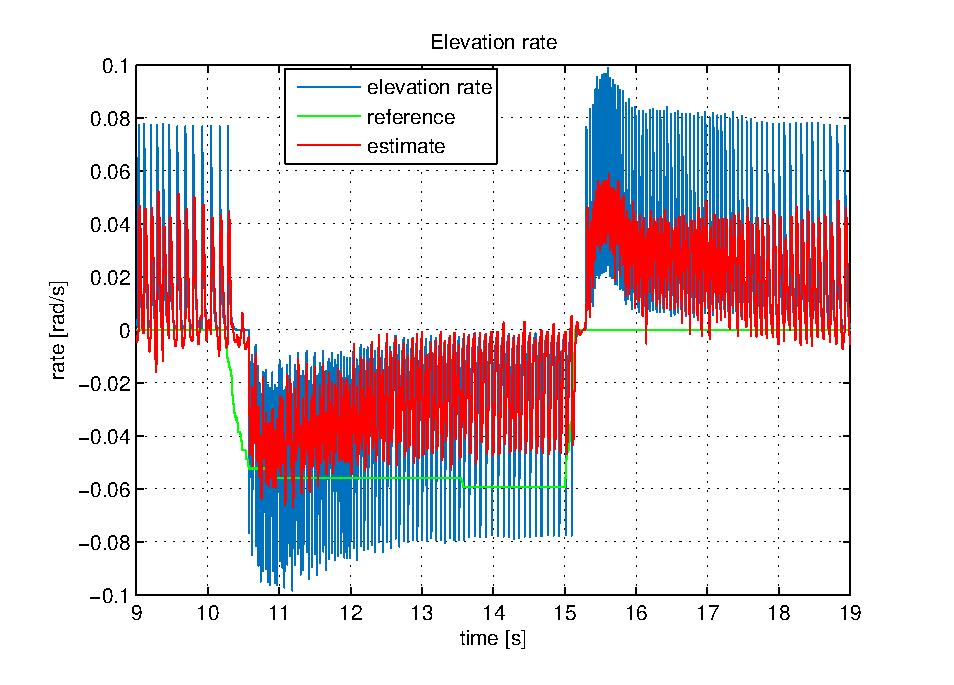
\includegraphics[width=0.9\textwidth]{plots/part4new/P/elevation_rate_60.eps}
	    \caption{Elevation rate with r = 60.}
        \label{fig:e_rate_60}
    \end{minipage}
\end{figure}

These three figures demonstrate what happens when the poles are placed either too close to the origin, just right, and too far away. \Cref{fig:e_rate_5} has the poles at $r=5$. This is not big enough for the estimator to predict the system fast enough. As we see on the plot it creates a phase lag, and this results in the system not staying at the reference, which is $0$. Our controller attempts to use the estimator to keep the system at the reference, when the estimator is too slow, the prediction will already have happened, meaning the controller is always reacting to late.\medskip

\Cref{fig:e_rate_60} shows the opposite behaviour, with poles with a too large radius. This plot shows the behaviour for $r=60$. Now the estimator is fast enough to predict the system. But where the small radius has a strong low filtering property, we see that this estimator doesn't. This causes a lot of noise on the estimator. A noisy estimator doesn't contribute anything useful to the system, and we didn't notice any big difference in the helicopter behaviour compared to the system without an estimator. Comparing the plots in \cref{fig:Elevationrate_pi} and the blue line in \cref{fig:e_rate_60}, also shows this behaviour.\medskip

The figure in the middles, \cref{fig:e_rate_27} show our final result. Here the poles are placed as shown in \cref{fig:pole_placement}, with a radius $r=27$. The estimator is fast enough to now predict the system, while still suppressing the noise from the elevation rate measurements by using its low pass characteristics.\medskip

\begin{figure}[H]
    \centering
	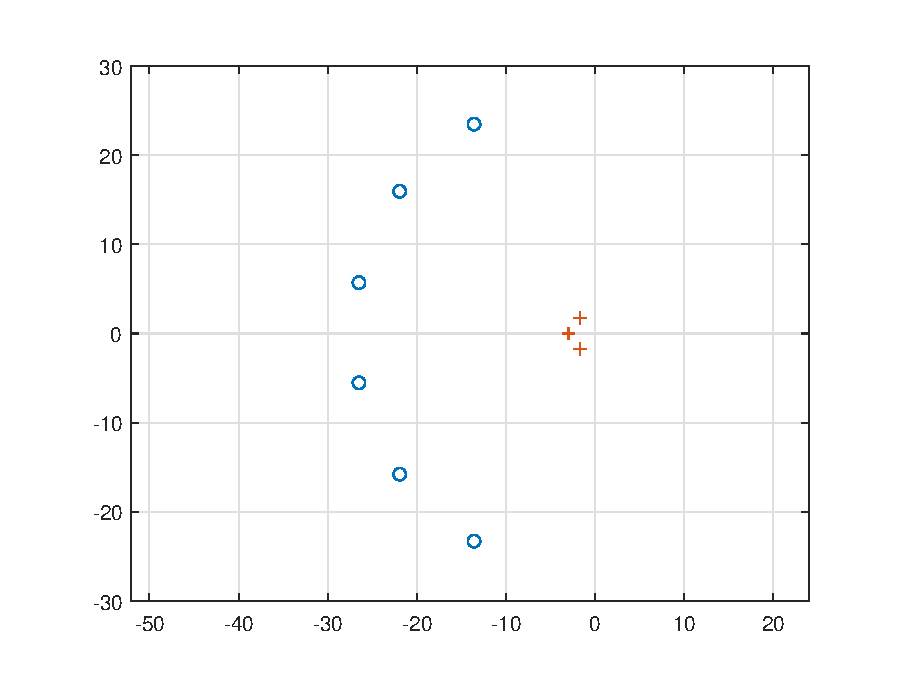
\includegraphics[width=0.9\linewidth]{plots/part4new/P/poles.eps}
    \caption{Pole placement for P controller. System poles:\textbf{\textcolor{red}{+}}, estimator poles:\textcolor{blue}{o}}

    \label{fig:pole_placement}
\end{figure}

We can further improve the system by implementing an integral effect as we did in part 3 problem 3. We found we got better results here by increasing the radius of the poles slightly and the final result of this can be seen in Figure \ref{fig:e_rate_42}.\\\medskip

\begin{figure}[H]
    \centering
	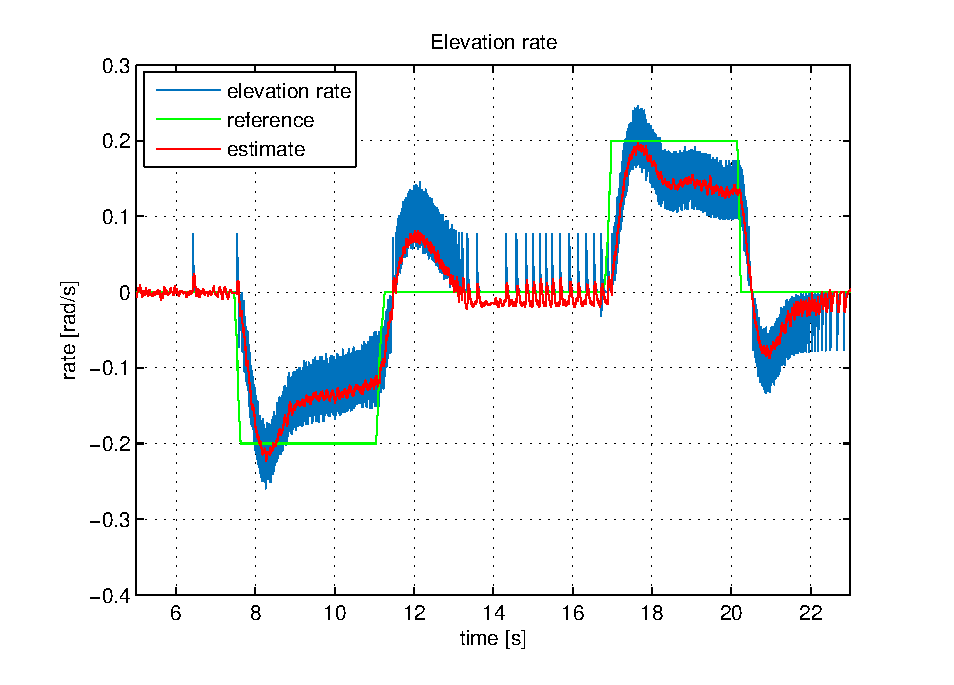
\includegraphics[width=0.9\linewidth]{plots/part4new/PI/e_rate_42.eps}
    \caption{Elevation rate with r = 42 and controller with integral effect}

    \label{fig:e_rate_42}
\end{figure}

%%%%%%%%%%%%%%%%%%%%%%%%%%%%%%%%%%%%%%%%%%%%%%%%%%%%%%%%%%%%%%%%%%%%%%%%%%%%%%%%%%%%%%%%%%%%

%%%%                                PART 4 PROBLEM 3

%%%%%%%%%%%%%%%%%%%%%%%%%%%%%%%%%%%%%%%%%%%%%%%%%%%%%%%%%%%%%%%%%%%%%%%%%%%%%%%%%%%%%%%%%%%%
\subsubsection{Problem 3}


In the final part of the lab assignment, our goal was to see whether we could use an estimator to control the system if we changed $y$. As shown in \cref{sec:P4p3}, only measuring pitch and elevation meant the system wouldn't be observable. However, by only measuring the elevation and travel, the system could be observed. This is because of the connection between travel and pitch, given by \cref{eq:model_linearized_lambda}. This allows the estimator to predict what the pitch is based on its knowledge of $\lambda$. \medskip

Even though the system is observable, it is harder to tune the controller. If the controller is to predict the pitch, it will need to differentiate the travel measurement, twice. It is a bad idea to differentiate a signal because differentiating noise creates even more, stronger noise. So differentiating noise twice isn't a good thing either.\medskip

\begin{figure}[H]
    \centering
	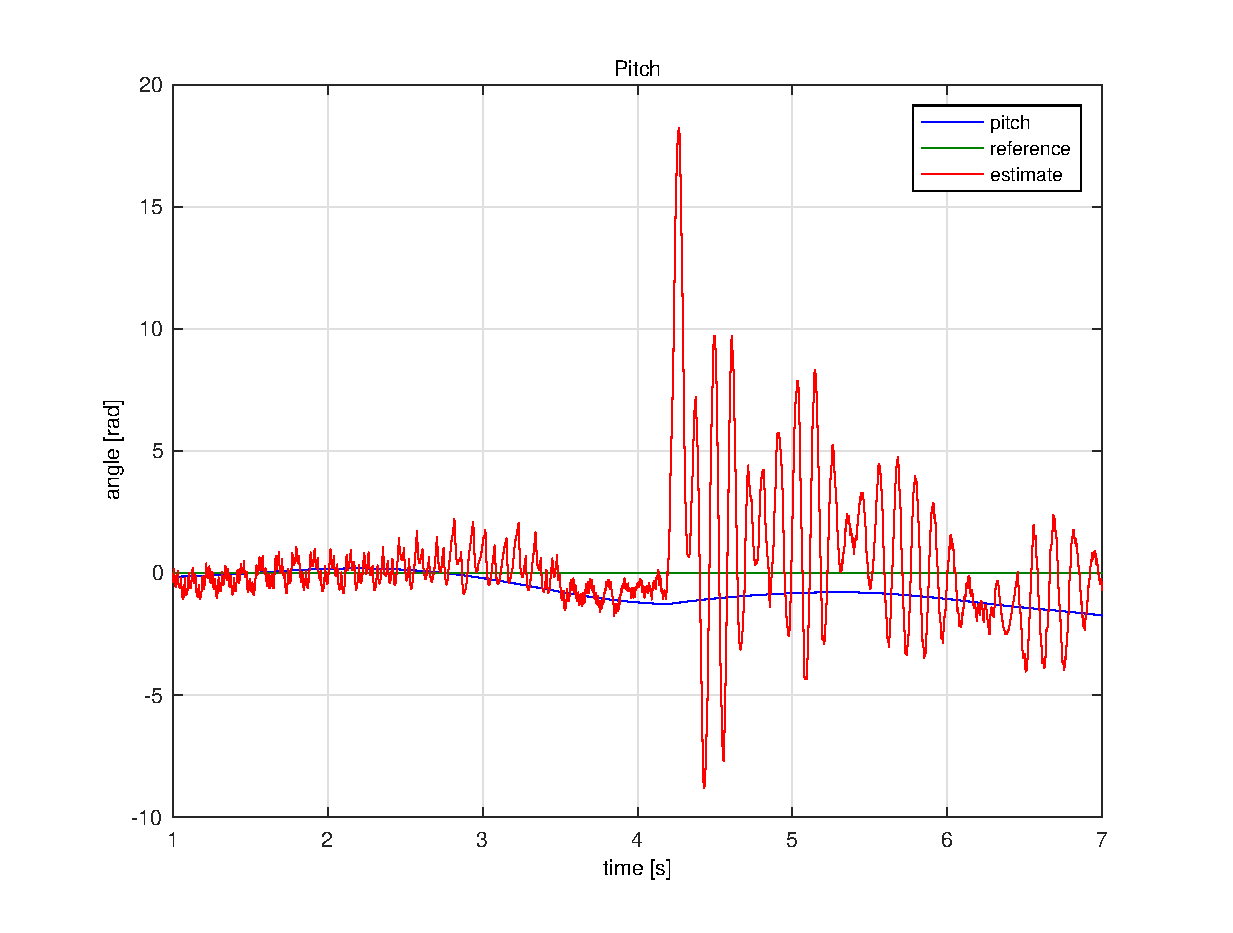
\includegraphics[width=0.9\linewidth]{plots/part4new/pitch_bad.eps}
    \caption{Pitch when pitch and elevation is measured.}
    \label{fig:BAD}
\end{figure}

\Cref{fig:BAD} shows this behaviour. The estimator thinks that the helicopter is swinging a lot around the $p$ joint, while it in reality is just leaning to one side. The controller uses the estimated value for control, and because of this, the system is hard to tune for pitch. The elevation is passed into the observer block, and is therefor easier to control.

When deciding how to tune the system we had to reduce the weight of the integrating factors dramatically as these produced an uncontrollable amount of noise, but we could not remove the entirely as steady state errors are expected when only being able to observe the travel to calculate the pitch. We also reduced the rest of the values in the system overall. The system is therefore slower, but when regulating a signal with a high amount of noise it is favorable that the system is ``sure'' of a change in pitch before responding. As the elevation estimated quite well the cost of regulating it is cheaper than regulating the pitch. The final \textbf{Q} and \textbf{R} can be seen in equations


\begin{equation} \label{eq:Q_P4p3}
    \bm{Q}_i = 
	\begin{bmatrix}
		150 &  0    &  0      &  0   &  0 \\
		0     &  10   &  0      &  0   &  0 \\
		0     &  0    &  150  &  0   &  0 \\
		0     &  0    &  0      &  10 &  0 \\
		0     &  0    &  0      &  0   &  10
	\end{bmatrix}
\end{equation} 

\begin{equation} \label{eq:R_P4p3}
    \bm{R}_i = 
	\begin{bmatrix}
		2   & 0  \\
		0    & 20\\

	\end{bmatrix}
\end{equation} 

The pole placement of the observer is also of paramount importance, and the system was highly sensitive to their placement. Poles at to close of a radius caused exponential oscillations, the observer is to slow to react to changes and the propellers simply vibrate at a high frequency. If the poles are to far away the integral effect causes the pitch and elevation to increase exponentially in one direction as the system is to slow to react to the estimated changes and the integral effect dominates. While tuning we found we got better responses by placing all poles close to each other on the real axis and settled on having the closest pole at -25.928\footnote{the system was so sensitive that three decimal places were necessary} and the other poles at 0.1 increments behind. The poles can be seen in Figure \ref{fig:P4p3_poles}.

\begin{figure}[H]
    \centering
	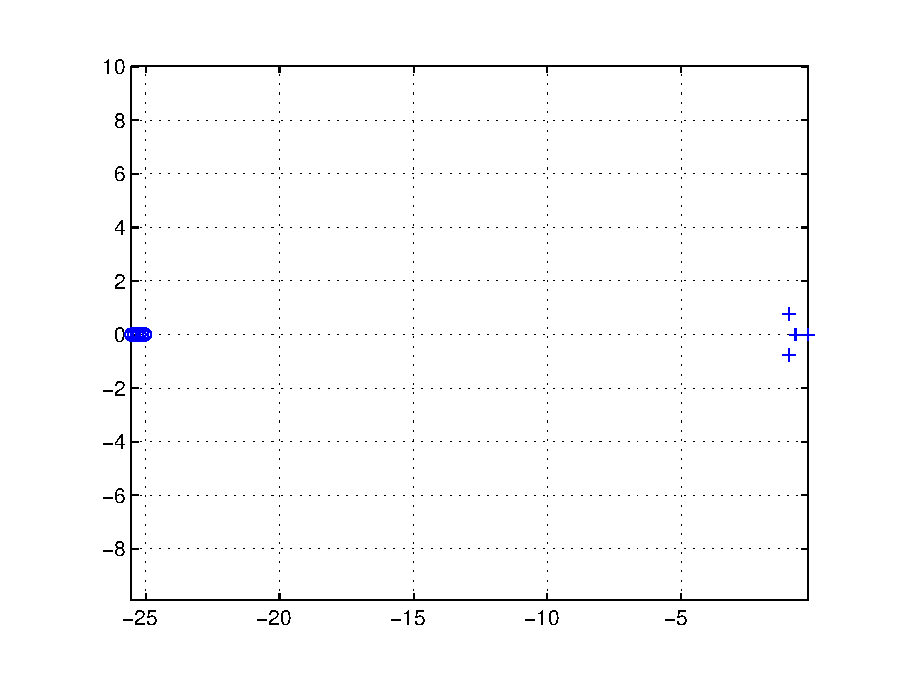
\includegraphics[width=0.9\linewidth]{plots/part4new/P4p3_poles.eps}
    \caption{Poles of the stable observer system}
    \label{fig:P4p3_poles}
\end{figure}

The final response of the system can be seen in Figure \ref{fig:P4p3_pitch}. 

\begin{figure}[H]
    \centering
	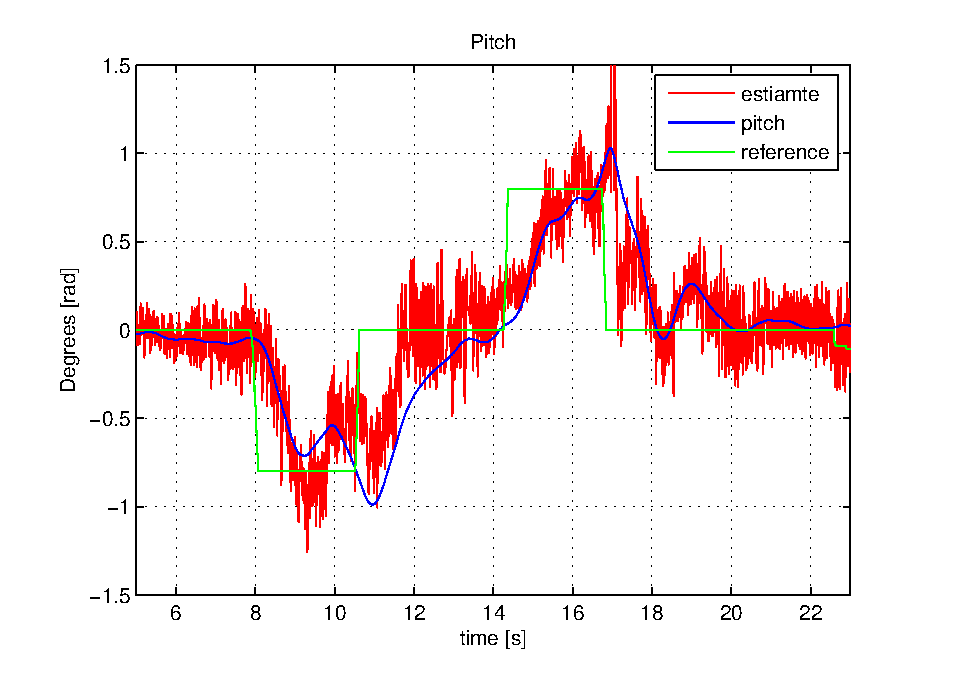
\includegraphics[width=0.9\linewidth]{plots/part4new/P4p3_bra_pitch.eps}
    \caption{Pitch of the system using the bad observer}
    \label{fig:P4p3_pitch}
\end{figure}

In conclusion; just because a system is observable for certain values it will not necessarily result in a well regulated system, it may be a good idea to apply a PBH test\footnote{Popov-Belevitch-Hautus test. Used to determine how controllable or observable a system is.} when one only has access to a limited number of states \cite{youtube}.

\newpage
